\documentclass[11pt,a4paper]{article}

% =============================================================================
%  MODULE 5A: MAGNETISM --- STUDENT COPY
%  PH7302: Condensed Matter Physics I  |  Department of Physics, NIT Calicut
% -----------------------------------------------------------------------------
%  Build:   pdflatex module5_student_copy.tex   (run twice for the ToC)
%  Figures: figures/*.pdf   (regenerate with:  python3 make_figures.py)
% =============================================================================

% --- Page Geometry -----------------------------------------------------------
\usepackage[a4paper, top=2.4cm, bottom=2.4cm, left=2.3cm, right=2.3cm,
            headheight=14pt]{geometry}

% --- Mathematics & Physics Packages ------------------------------------------
\usepackage{amsmath, amssymb, amsfonts, bm, mathtools}

% --- Tables, Lists & Typography ----------------------------------------------
\usepackage{booktabs, longtable, array, tabularx}
% Ragged-right table columns: justified p-columns in narrow columns stretch
% the inter-word spacing badly (e.g. "Orbital   Larmor   shielding").
\renewcommand{\tabularxcolumn}[1]{p{#1}}
\newcolumntype{L}[1]{>{\raggedright\arraybackslash}p{#1}}
\newcolumntype{Y}{>{\raggedright\arraybackslash}X}
\usepackage{enumitem}
\usepackage{microtype}
\usepackage{caption}
\usepackage{listings}

% --- Graphics & Colour --------------------------------------------------------
\usepackage{graphicx}
\usepackage{xcolor}
\definecolor{primary}{RGB}{20, 50, 100}     % deep blue  (main accents)
\definecolor{secondary}{RGB}{140, 40, 30}   % brick red  (highlight)
\definecolor{tealcol}{RGB}{17, 122, 101}
\definecolor{orangecol}{RGB}{199, 124, 2}
\definecolor{purplecol}{RGB}{106, 61, 154}

% --- Native Vector Graphics ----------------------------------------------------
\usepackage{tikz}
\usetikzlibrary{arrows.meta, calc, decorations.pathmorphing,
                decorations.pathreplacing, patterns, positioning}

% --- Boxed Environments for Student Learning ----------------------------------
\usepackage[most]{tcolorbox}
\tcbuselibrary{breakable, skins}

% --- Running Headers & Footers ------------------------------------------------
\usepackage{fancyhdr}
\usepackage{lastpage}
\pagestyle{fancy}
\fancyhf{}
\fancyhead[L]{\small\color{primary}\textbf{PH7302: Condensed Matter Physics}}
\fancyhead[R]{\small\color{gray!75!black}Module 5A: Magnetism (Student Copy)}
\fancyfoot[C]{\small\thepage\ \textcolor{gray!75!black}{of~\pageref{LastPage}}}
\renewcommand{\headrulewidth}{0.5pt}
\renewcommand{\footrulewidth}{0.4pt}

% --- Section Title Styling ----------------------------------------------------
\usepackage{titlesec}
\titleformat{\section}{\large\bfseries\color{primary}}{\thesection}{1em}{}[\titlerule]
\titleformat{\subsection}{\normalsize\bfseries\color{primary!75!black}}{\thesubsection}{1em}{}
\titleformat{\subsubsection}{\small\bfseries\color{black}}{\thesubsubsection}{1em}{}

% --- Hyperlinks ----------------------------------------------------------------
\usepackage{hyperref}
\hypersetup{
    colorlinks=true,
    linkcolor=primary,
    citecolor=primary,
    urlcolor=secondary,
    pdfauthor={Department of Physics, National Institute of Technology Calicut},
    pdftitle={Module 5A: Magnetism --- Student Copy},
    pdfsubject={PH7302 Condensed Matter Physics I}
}

% --- Table of Contents (tightened so it fits on a single page) ---------------
%     tocloft must be loaded after hyperref.
\usepackage{tocloft}
\setlength{\cftbeforesecskip}{2.2pt}
\setlength{\cftbeforesubsecskip}{0.6pt}
\renewcommand{\cftsecfont}{\bfseries\color{primary}}
\renewcommand{\cftsubsecfont}{\normalfont\color{black}}
\renewcommand{\cftsecpagefont}{\bfseries\color{primary}}

% =============================================================================
%  STUDENT LEARNING BOXES  (replacing the instructor prompts of the original)
% =============================================================================
% 1. Conceptual Checkpoint
\newtcolorbox{checkpointbox}[1]{%
    colback=blue!3!white, colframe=primary,
    fonttitle=\bfseries\small, title={Conceptual Checkpoint: #1},
    arc=2mm, boxrule=0.9pt, breakable, enhanced,
    before upper={\parindent0pt}
}

% 2. Study Takeaway
\newtcolorbox{takeawaybox}[1]{%
    colback=teal!4!white, colframe=tealcol,
    fonttitle=\bfseries\small, title={Study Takeaway: #1},
    arc=2mm, boxrule=0.9pt, breakable, enhanced,
    before upper={\parindent0pt}
}

% 3. Problem-Solving Strategy
\newtcolorbox{methodbox}[1]{%
    colback=purple!4!white, colframe=purplecol,
    fonttitle=\bfseries\small, title={Problem-Solving Strategy: #1},
    arc=2mm, boxrule=0.9pt, breakable, enhanced,
    before upper={\parindent0pt}
}

% 4. Common Misconception & Pitfall
\newtcolorbox{pitfallbox}[1]{%
    colback=orange!5!white, colframe=orangecol,
    fonttitle=\bfseries\small, title={Common Misconception \& Pitfall: #1},
    arc=2mm, boxrule=0.9pt, breakable, enhanced,
    before upper={\parindent0pt}
}

% 5. In-Text Worked Example
\newtcolorbox{examplebox}[2]{%
    colback=gray!4!white, colframe=primary!70!black,
    fonttitle=\bfseries\small, title={Worked Example: #1},
    label={#2},
    arc=2mm, boxrule=1.0pt, breakable, enhanced,
    before upper={\parindent0pt}
}

% 6. Upfront Assignment Part Box
\newtcolorbox{assignmentbox}[1]{%
    colback=blue!2!white, colframe=primary,
    fonttitle=\bfseries\normalsize, title={#1},
    arc=2mm, boxrule=1.0pt, breakable, enhanced,
    before upper={\parindent0pt}
}

% 7. Key Equation (results that must be memorised)
\newtcolorbox{keyeqbox}[1]{%
    colback=primary!3!white, colframe=primary!85!black,
    fonttitle=\bfseries\small, title={Key Result: #1},
    arc=2mm, boxrule=0.9pt, breakable, enhanced,
    before upper={\parindent0pt}
}

% 8. Formal definition
\newtcolorbox{definitionbox}[1]{%
    colback=gray!4!white, colframe=black!65,
    fonttitle=\bfseries\small, title={#1},
    arc=2mm, boxrule=0.9pt, breakable, enhanced,
    before upper={\parindent0pt}
}

% 9. Figure caption / sketch guide
\newtcolorbox{sketchbox}[1]{%
    colback=gray!3!white, colframe=gray!55!black,
    fonttitle=\bfseries\small, title={How to Read This Figure: #1},
    arc=2mm, boxrule=0.8pt, breakable, enhanced,
    before upper={\parindent0pt}
}

% 10. Out-of-Syllabus / Optional Enrichment Callout
\newcommand{\extratag}{\hfill\mbox{\normalfont\footnotesize\sffamily\color{secondary}\textbf{[Optional / Advanced Read]}}}
\newtcolorbox{enrichmentnote}[1]{%
    colback=purple!3!white, colframe=purplecol!80!black,
    fonttitle=\bfseries\small, title={Optional Enrichment / Beyond-Syllabus Read: #1},
    arc=2mm, boxrule=0.9pt, breakable, enhanced,
    before upper={\parindent0pt}
}

% --- Listings Style (Python appendix) -----------------------------------------
\definecolor{codebg}{RGB}{247, 248, 250}
\definecolor{codeframe}{RGB}{200, 206, 214}
\definecolor{codetext}{RGB}{35, 40, 48}
\lstset{
    language=Python,
    backgroundcolor=\color{codebg},
    frame=single, rulecolor=\color{codeframe},
    basicstyle=\ttfamily\footnotesize\color{codetext},
    breaklines=true,
    keywordstyle=\color{primary!85!black}\bfseries,
    commentstyle=\color{tealcol!75!black}\itshape,
    stringstyle=\color{secondary!80!black},
    numbers=left, numberstyle=\tiny\color{gray!70!black}, numbersep=8pt,
    tabsize=4, showstringspaces=false,
    framexleftmargin=24pt
}

% --- Custom Macros --------------------------------------------------------------
\newcommand{\vb}[1]{\mathbf{#1}}
\newcommand{\ket}[1]{\left|#1\right\rangle}
\newcommand{\bra}[1]{\left\langle #1\right|}
\newcommand{\braket}[2]{\left\langle #1 \middle| #2 \right\rangle}
\newcommand{\dd}{\,\mathrm{d}}
\newcommand{\e}{\mathrm{e}}
\newcommand{\amuB}{\mu_{\mathrm{B}}}
\newcommand{\Ang}{\text{\AA}}

\begin{document}

% =============================================================================
%  TITLE BLOCK
% =============================================================================
\title{%
    \vspace{-1.5cm}
    \textbf{\LARGE Module 5A: Magnetism}\\[0.35cm]
    \Large Student Copy --- Comprehensive Lecture \& Tutorial Guide\\[0.25cm]
    \large\color{primary}\textbf{PH7302: Condensed Matter Physics I}
}
\author{%
    \textbf{Department of Physics}\\
    \text{National Institute of Technology Calicut}
}
\date{Academic Year 2026--2027}
\maketitle

\vspace{-0.6cm}
\begin{abstract}
\noindent
This document is the complete, self-contained student edition of \textbf{Module 5A: Magnetism} for PH7302 Condensed Matter Physics I (Department of Physics, NIT Calicut). It develops the magnetic properties of solids from foundational definitions of magnetisation, magnetostatic units and the Bohr--van Leeuwen theorem, through atomic diamagnetism (Langevin/Larmor theory and the quantum diamagnetic Hamiltonian), localised paramagnetism (Hund's rules, Land\'e $g$-factor, orbital quenching, Brillouin function and Curie's law) and itinerant paramagnetism (Pauli spin susceptibility and Landau diamagnetism). The second half treats the exchange interaction (Heitler--London $\mathrm{H}_2$ model, Heisenberg Hamiltonian, direct, superexchange and RKKY mechanisms) and collective ordering: Weiss molecular-field theory, the Curie--Weiss law, spontaneous magnetisation, and the two-sublattice N\'eel model for antiferromagnetism. Advanced extension topics (Van Vleck paramagnetism, adiabatic demagnetisation, the Stoner criterion, magnons, domain walls, hysteresis, and ferrimagnetism) are explicitly demarcated with \textbf{[Optional / Advanced Read]} tags so students can distinguish core exam syllabus material from advanced enrichment. Dielectric, ferroelectric, piezoelectric and optical properties of solids will be covered in companion guide \textbf{Module 5B}. The edition features an upfront assignment of 24 curated problems with final answers, 3 fully solved in-text numerical derivations, 20+ targeted learning boxes, four vector data figures, a master comparison table, a symbol glossary, and reproducible Python verification scripts.
\end{abstract}

\vspace{0.3cm}

% =============================================================================
%  HOW TO USE THIS STUDENT EDITION
% =============================================================================
\section*{How to Use This Student Edition}
\addcontentsline{toc}{section}{How to Use This Student Edition}

This student edition is designed to take you from first principles to exam-ready command of magnetism. The material is dense in algebra but light in intuition, so the edition leans heavily on physical pictures, worked numbers and explicit checkpoints. Work through it in the following way.

\begin{enumerate}[leftmargin=*]
    \item \textbf{Distinguish Core Syllabus from Optional Enrichment.} Sections, sub-topics and assignment problems tagged with \textbf{[Optional / Advanced Read]} contain enriching physical applications and derivations (e.g.\ Van Vleck paramagnetism, adiabatic demagnetisation, Stoner band splitting, spin-wave heat capacity, Bloch walls, and ferrimagnets). These topics go beyond the compulsory PH7302 semester exam syllabus and are provided for physical completeness and competitive exam preparation (such as CSIR-NET / GATE). Non-interested students can safely skip them without losing syllabus marks.
    \item \textbf{Attempt the Upfront Assignment Continuously.} The section immediately after the Table of Contents contains the complete Module 5A problem set, organised into six thematic parts that map onto the chapters below. Each problem states exact parameters and ends with the expected final answer or a short hint in brackets (\texttt{[Ans: ...]}). Attempt each problem as soon as you finish the corresponding chapter --- do not save them all for the end.
    \item \textbf{Study the In-Text Worked Examples.} Three fully solved model derivations are embedded in the chapters at the points where the relevant technique is introduced (atomic hydrogen diamagnetism, the exchange field of iron, and magnon heat capacity). Every one of them is written out in SI units with the unit conversions shown explicitly. Cover the solution, work it yourself, then compare.
    \item \textbf{Engage with the Learning Boxes.} Distinct box types appear throughout and each serves a specific purpose:
    \begin{itemize}[leftmargin=1.5cm]
        \item \textbf{Conceptual Checkpoints}: quick tests of understanding that expose the gap between recognising a formula and understanding it.
        \item \textbf{Study Takeaways}: the one-sentence physical statements worth committing to memory.
        \item \textbf{Problem-Solving Strategies}: systematic calculation recipes for recurring exam question types.
        \item \textbf{Common Misconceptions \& Pitfalls}: the traps that cost marks --- especially the SI/CGS unit traps, which dominate this module.
        \item \textbf{Key Results}: boxed equations that you should be able to reproduce from memory.
    \end{itemize}
    \item \textbf{Read the Figures as Arguments.} The four generated figures are not decoration: each one isolates a piece of physics that is hard to see from the algebra alone. The captions tell you what to look for.
    \item \textbf{Reproduce the Computations.} Appendix~A contains the complete Python source for all four figures. Running and modifying these scripts converts the qualitative statements of the text into quantitative intuition --- and it is the fastest way to check whether you have really understood the Brillouin function or the Curie--Weiss law.
\end{enumerate}

\vspace{0.3cm}

% =============================================================================
%  MODULE OVERVIEW
% =============================================================================
\section{Module Overview and Syllabus Alignment}
\label{sec:overview}

The structure of this module and the syllabus learning outcomes that it addresses are summarised in Table~\ref{tab:syllabus_map}.

\begin{table}[ht]
\centering
\small
\renewcommand{\arraystretch}{0.98}
\begin{tabular}{L{1.8cm} L{3.9cm} L{8.9cm}}
\toprule
\textbf{Chapter} & \textbf{Core Topic} & \textbf{Key Learning Outcomes \& Syllabus Role} \\
\midrule
\textbf{Ch.\ 1} & Foundations, Units and the Bohr--van Leeuwen Theorem & \textbf{[Core]} Magnetisation, $\vb{B}$/$\vb{H}$/$\vb{M}$ in SI and CGS; susceptibility and molar susceptibility; proof that classical mechanics predicts zero magnetisation. \\
\textbf{Ch.\ 2} & Atomic Diamagnetism & \textbf{[Core]} Larmor precession and the Langevin classical result; quantum diamagnetic Hamiltonian; closed-shell atoms; noble-gas trends. \\
\textbf{Ch.\ 3} & Localised Paramagnetism & \textbf{[Core]} Land\'e $g$-factor; Hund's rules; Brillouin function; Curie law; orbital quenching in $3d$ vs.\ $4f$. \emph{(Sec.~3.5 Van Vleck is an Optional Read)}. \\
\textbf{Ch.\ 4} & Itinerant Paramagnetism & \textbf{[Core]} Pauli exclusion principle; Pauli spin susceptibility; Landau diamagnetism. \emph{(Sec.~4.3 Adiabatic Demagnetisation is an Optional Read)}. \\
\textbf{Ch.\ 5} & The Exchange Interaction & \textbf{[Core]} Failure of dipolar interaction; Heitler--London $\text{H}_2$ model; singlet/triplet splitting; Heisenberg Hamiltonian; exchange mechanisms. \\
\textbf{Ch.\ 6} & Ferromagnetism & \textbf{[Core]} Weiss molecular-field theory; Curie--Weiss law and $T_C$; spontaneous magnetisation and $\beta = 1/2$. \emph{(Sec.~6.4 Stoner criterion is an Optional Read)}. \\
\textbf{Ch.\ 7} & Magnons, Domains and Hysteresis & \textbf{[Optional / Extension]} Magnon dispersion; Bloch's $T^{3/2}$ law; magnetostatic energy; Bloch-wall width; hysteresis loops. \\
\textbf{Ch.\ 8} & Antiferromagnetism and Ferrimagnetism & \textbf{[Core AFM]} Two-sublattice N\'eel model; $T_N = \mu C$; $\chi = 2C/(T+T_N)$; $\chi_\parallel$ vs.\ $\chi_\perp$ and the $T_N$ cusp. \emph{(Sec.~8.3 Ferrimagnetism is an Optional Read)}. \\
\textbf{Ch.\ 9} & Synthesis and Formula Sheet & \textbf{[Core Revision]} Master comparison of magnetic classes; consolidated formula sheet for exam revision. \\
\bottomrule
\end{tabular}
\caption{Structure, syllabus coverage and learning outcomes for Module 5A (Magnetism). Note: Companion topics in Module 5 (Dielectrics, Ferroelectrics, Piezoelectrics \& Optical Properties) are covered in Module 5B.}
\label{tab:syllabus_map}
\end{table}

\begin{enrichmentnote}{Curriculum Scope: Module 5A versus Module 5B}
In the official NIT Calicut PH7302 syllabus, Module 5 encompasses:
\begin{center}
\textit{"Dielectric properties of insulators -- Piezoelectric and Ferroelectric materials -- Optical properties of solids -- Magnetism-exchange interaction, diamagnetism, paramagnetism, ferromagnetism and antiferromagnetism."}
\end{center}
This document constitutes \textbf{Module 5A}, dedicated entirely to the magnetic properties. The dielectric, ferroelectric, piezoelectric and optical properties will be issued in companion guide \textbf{Module 5B}. Within Module 5A, sections tagged \textbf{[Optional / Advanced Read]} extend beyond the minimum compulsory syllabus and may be omitted by students focusing solely on semester exam essentials.
\end{enrichmentnote}

Magnetism is the one branch of condensed matter physics in which the classical and quantum worlds give qualitatively opposite answers. The thread running through this module is that \emph{charge} motion produces only a vanishingly small diamagnetic response (the Bohr--van Leeuwen theorem), whereas \emph{spin} and \emph{quantised orbital motion} produce the entire palette of magnetic behaviour, from the $10^{-6}$ diamagnetism of copper to the $10^{5}$ paramagnetism of a ferromagnet.

% =============================================================================
%  CONSTANTS, UNITS AND NOTATION
% =============================================================================
\section{Physical Constants, Units and Notation}
\label{sec:constants}

\subsection{Constants Used Throughout}

\begin{table}[ht]
\centering
\small
\renewcommand{\arraystretch}{1.2}
\begin{tabular}{llll}
\toprule
\textbf{Quantity} & \textbf{Symbol} & \textbf{SI Value} & \textbf{CGS Value} \\
\midrule
Planck constant & $h$ & $6.6261\times10^{-34}\ \mathrm{J\,s}$ & $6.6261\times10^{-27}\ \mathrm{erg\,s}$ \\
Reduced Planck constant & $\hbar$ & $1.0546\times10^{-34}\ \mathrm{J\,s}$ & $1.0546\times10^{-27}\ \mathrm{erg\,s}$ \\
Electron mass & $m_e$ & $9.1094\times10^{-31}\ \mathrm{kg}$ & $9.1094\times10^{-28}\ \mathrm{g}$ \\
Elementary charge & $e$ & $1.6022\times10^{-19}\ \mathrm{C}$ & $4.8032\times10^{-10}\ \mathrm{statC}$ \\
Boltzmann constant & $k_B$ & $1.3807\times10^{-23}\ \mathrm{J/K}$ & $1.3807\times10^{-16}\ \mathrm{erg/K}$ \\
Avogadro constant & $N_A$ & $6.0221\times10^{23}\ \mathrm{mol^{-1}}$ & --- \\
Bohr magneton & $\mu_B = e\hbar/2m_e$ & $9.2740\times10^{-24}\ \mathrm{J/T}$ & $9.2740\times10^{-21}\ \mathrm{erg/G}$ \\
Bohr magneton (in eV) & $\mu_B$ & $5.7884\times10^{-5}\ \mathrm{eV/T}$ & --- \\
Permeability of vacuum & $\mu_0$ & $4\pi\times10^{-7}\ \mathrm{H/m}$ & $1$ (Gaussian) \\
Electron gyromagnetic ratio & $g$ & $\approx 2.0023$ & $\approx 2.0023$ \\
Bohr radius & $a_0$ & $5.2918\times10^{-11}\ \mathrm{m}$ & $5.2918\times10^{-9}\ \mathrm{cm}$ \\
\bottomrule
\end{tabular}
\caption{Fundamental constants used in this module, in both unit systems.}
\label{tab:constants}
\end{table}

\subsection*{Useful Numerical Benchmarks}
\begin{itemize}[leftmargin=1.5cm]
    \item $1\ \mathrm{eV} = 1.6022\times10^{-19}\ \mathrm{J}$; hence $1\ \mathrm{meV} = 1.6022\times10^{-22}\ \mathrm{J}$.
    \item Thermal energy at room temperature: $k_B T = 0.02585\ \mathrm{eV}$ at $T = 300\ \mathrm{K}$.
    \item At $T = 300\ \mathrm{K}$ and $B = 1\ \mathrm{T}$: $\mu_B B/k_BT = (5.788\times10^{-5}\ \mathrm{eV})/(0.02585\ \mathrm{eV}) = 2.24\times10^{-3}$, so the dimensionless field is $x = g_JJ\times2.24\times10^{-3}\ll1$ for any realistic ion. This is why the weak-field (Curie) limit is the normal laboratory situation, and why it takes a strong magnet or a very low temperature to reach saturation.
    \item Fermi temperature of typical metals: $T_F \sim 5\times10^{4}$--$10^{5}\ \mathrm{K}$, so conduction electrons are essentially degenerate at room temperature.
    \item Curie temperature of iron: $T_C = 1043\ \mathrm{K}$, i.e.\ $k_B T_C \approx 0.090\ \mathrm{eV}$.
    \item $1\ \mathrm{T} = 10^{4}\ \mathrm{G}$ and $\mu_0 = 4\pi\times10^{-7}\ \mathrm{T\,m/A}$.
\end{itemize}

\subsection*{Field and Susceptibility Conventions --- Read This Before Chapter 6}

Magnetism is the classic source of lost marks through unit confusion. Kittel and Ashcroft \& Mermin write in Gaussian (CGS) units, while most modern papers and instruments use SI. This edition is explicit about which is in use at every step.

\begin{table}[ht]
\centering
\small
\renewcommand{\arraystretch}{1.2}
\begin{tabular}{L{4.4cm} L{5.0cm} L{5.3cm}}
\toprule
\textbf{Quantity} & \textbf{SI} & \textbf{CGS (Gaussian)} \\
\midrule
Constitutive relation & $\vb{B} = \mu_0(\vb{H} + \vb{M})$ & $\vb{B} = \vb{H} + 4\pi\vb{M}$ \\
Volume susceptibility & $\chi = \partial M/\partial H \approx \mu_0 M/B$ & $\chi = \partial M/\partial H \approx M/B$ \\
Relation between the two & \multicolumn{2}{c}{$\chi_{\mathrm{SI}} = 4\pi\,\chi_{\mathrm{CGS}}$ \quad (same physical sample)} \\
Molar susceptibility definition & $\chi_M^{\mathrm{SI}} = \chi_{\mathrm{SI}}\,V_m^{\mathrm{SI}}$ & $\chi_M^{\mathrm{CGS}} = \chi_{\mathrm{CGS}}\,V_m^{\mathrm{CGS}}$ \\
Molar conversion relation & \multicolumn{2}{c}{$\chi_M^{\mathrm{SI}} = 4\pi\times 10^{-6}\,\chi_M^{\mathrm{CGS}}$ \quad ($\chi_M^{\mathrm{SI}}$ in $\mathrm{m^3/mol}$, $\chi_M^{\mathrm{CGS}}$ in $\mathrm{cm^3/mol}$)} \\
Bohr magneton & $9.274\times10^{-24}\ \mathrm{J/T}$ & $9.274\times10^{-21}\ \mathrm{erg/G}$ \\
Molar susceptibility unit & $\mathrm{m^3/mol}$ & $\mathrm{cm^3/mol}$ \\
\bottomrule
\end{tabular}
\caption{Field and susceptibility conventions in the two unit systems used in this module.}
\label{tab:units}
\end{table}

\begin{pitfallbox}{The SI/CGS trap in this module}
The SI and CGS magnetisation equations look almost identical but are \emph{not}:
\[
\text{SI:}\quad \chi = \frac{\mu_0 M}{B},
\qquad
\text{CGS:}\quad \chi = \frac{M}{B}.
\]
In SI the permeability $\mu_0$ appears in $\chi$, in CGS a factor $4\pi$ appears in $\vb{B}=\vb{H}+4\pi\vb{M}$, and the dimensionless volume susceptibilities satisfy $\chi_{\mathrm{SI}} = 4\pi\,\chi_{\mathrm{CGS}}$.

\textbf{Molar susceptibility conversion.} Because volume susceptibility contains that factor of $4\pi$, the molar susceptibility conversion also involves $4\pi$:
\[
\chi_M^{\mathrm{SI}} = \chi_{\mathrm{SI}}\,V_m^{\mathrm{SI}} = (4\pi\,\chi_{\mathrm{CGS}})(10^{-6}\,V_m^{\mathrm{CGS}}) = 4\pi\times 10^{-6}\,\chi_M^{\mathrm{CGS}}.
\]
A classic examination error is simply multiplying $\chi_M^{\mathrm{CGS}}$ by $10^{-6}$ while omitting the $4\pi$, which leaves the SI molar susceptibility an order of magnitude too small!

\textbf{Convention adopted in this edition.} Chapters 1--5 use SI. From Chapter 6 onwards the mean-field (Weiss, N\'eel, ferrimagnet) derivations are carried out in \textbf{CGS}, following Kittel, because it keeps the algebra clean:
\[
M = \frac{C}{T}\left(H_a + \lambda M\right)
\quad\Longrightarrow\quad
\chi = \frac{C}{T - T_C},
\qquad
T_C = \lambda C = \frac{2zJS(S+1)}{3k_B}.
\]
Whenever an SI form is needed it is given alongside. Every answer in the assignment set states its unit system.
\end{pitfallbox}

\clearpage

% =============================================================================
%  TABLE OF CONTENTS
% =============================================================================
\tableofcontents
\clearpage
% =============================================================================
%  UPFRONT ASSIGNMENT: MODULE 5A
% =============================================================================
\section*{Assignment: Module 5A --- Magnetism}
\addcontentsline{toc}{section}{Assignment: Module 5A --- Practice Problems Set}
\label{sec:assignment_module5}

\noindent\fbox{%
\parbox{\dimexpr\textwidth-2\fboxsep-2\fboxrule\relax}{%
\small
\textbf{Instructions to Students.} This assignment covers the derivations, physical concepts and quantitative techniques developed across Module 5A. The problems are grouped into six thematic parts that follow the chapter order of this guide. Problems marked with \textbf{[Optional / Advanced Read]} address extension topics and may be skipped by students focusing only on compulsory semester exam questions. Each problem supplies exact parameters and closes with the expected final answer or an essential hint in square brackets (\texttt{[Ans: ...]}). Full step-by-step model derivations for the recurring problem archetypes appear as \emph{Worked Examples} inside the corresponding chapters --- attempt each problem before turning to them. State the unit system (SI or CGS) in every answer. Unless told otherwise, use $m_e = 9.1094\times10^{-31}\ \mathrm{kg}$, $e = 1.6022\times10^{-19}\ \mathrm{C}$, $\mu_0 = 4\pi\times10^{-7}\ \mathrm{H/m}$ and $k_B = 1.3807\times10^{-23}\ \mathrm{J/K}$.
}%
}

\vspace{0.4cm}

% ---------------------------------------------------------------------------
\begin{assignmentbox}{Part I: Foundations, Units and Atomic Diamagnetism}
\begin{enumerate}[label=\textbf{I.\arabic*.}, leftmargin=*]
    \item \textbf{Converting between CGS and SI susceptibilities.}\\
    A solid specimen has a Gaussian volume susceptibility $\chi_{\mathrm{CGS}} = -4.5\times10^{-6}$ and a density $\rho = 9.2\ \mathrm{g\,cm^{-3}}$ with molar mass $M_{\mathrm{mol}} = 184.7\ \mathrm{g\,mol^{-1}}$.
    \begin{enumerate}[label=(\alph*)]
        \item Convert to the SI volume susceptibility.
        \item Compute the molar susceptibility $\chi_M$ in $\mathrm{cm^3/mol}$.
        \item Compute the molar susceptibility in SI units, $\mathrm{m^3/mol}$.
    \end{enumerate}
    \textbf{[Ans:} (a) $\chi_{\mathrm{SI}} = 4\pi\chi_{\mathrm{CGS}} = -5.65\times10^{-5}$; (b) $V_m = M_{\mathrm{mol}}/\rho = 20.08\ \mathrm{cm^3/mol}$, so $\chi_M^{\mathrm{CGS}} = \chi_{\mathrm{CGS}}V_m = -9.04\times10^{-5}\ \mathrm{cm^3/mol}$; (c) $\chi_M^{\mathrm{SI}} = \chi_{\mathrm{SI}}V_m^{\mathrm{SI}} = 4\pi\times 10^{-6}\chi_M^{\mathrm{CGS}} = -1.135\times10^{-9}\ \mathrm{m^3/mol}$ (remember the factor of $4\pi$ must be included when converting to SI)\textbf{]}

    \item \textbf{Langevin diamagnetic susceptibility of a many-electron atom.}\\
    An atom carries $Z = 3$ bound electrons with mean-square radius $\langle r^2\rangle = 0.45\ \Ang^2$, and the sample has $N = 6.0\times10^{28}$ atoms per cubic metre. Compute the volume diamagnetic susceptibility in SI.
    \textbf{[Ans:} $\chi_{\mathrm{dia}} = -\mu_0 NZ e^2\langle r^2\rangle/6m_e = -4.78\times10^{-6}$ (dimensionless, SI)\textbf{]}

    \item \textbf{Atomic hydrogen: complete the Bohr calculation.}\\
    Using $\psi_{1s} = (\pi a_0^3)^{-1/2}e^{-r/a_0}$ with $a_0 = 0.529\ \Ang$, show that $\langle r^2\rangle = 3a_0^2$ and calculate the molar diamagnetic susceptibility of atomic hydrogen.
    \textbf{[Ans:} $\langle r^2\rangle = 3a_0^2 = 8.40\times10^{-17}\ \mathrm{cm^2}$; $\chi_M = -\mu_0 N_A e^2a_0^2/2m_e = -2.98\times10^{-11}\ \mathrm{m^3/mol} = -2.37\times10^{-6}\ \mathrm{cm^3/mol}$ (CGS molar)\textbf{]}

    \item \textbf{Larmor precession and the induced moment.}\\
    An electron with mean-square transverse radius $\langle\rho^2\rangle = 0.30\ \Ang^2$ is placed in a perpendicular field $B = 2.0\ \mathrm{T}$. Compute (a) the induced magnetic moment per atom and (b) the induced current.
    \textbf{[Ans:} (a) $\mu_{\mathrm{ind}} = -\frac{Ze^2B}{4m_e}\langle\rho^2\rangle = -4.23\times10^{-29}\ \mathrm{J/T}$; (b) with $A = \pi\langle\rho^2\rangle = 9.42\times10^{-21}\ \mathrm{m^2}$, $I = \mu/A = -4.48\times10^{-9}\ \mathrm{A}$ (equivalently $I = -Ze^2B/4\pi m_e$)\textbf{]}

    \item \textbf{The Bohr--van Leeuwen theorem, stated and defended.}\\
    (a) Write the classical canonical partition function for $N$ particles of charge $q_i$ in a vector potential $\vb{A}(\vb{r})$ with $\vb{B} = \nabla\times\vb{A}$.
    (b) Show explicitly, by shifting the integration variable, that $Z$ does not depend on $\vb{B}$.
    (c) Explain in one sentence what physical cancellation the algebra encodes.
    \textbf{[Ans:} (a) $Z = \frac{1}{N!h^{3N}}\int d^{3N}r\,d^{3N}p\,\exp[-\frac{\beta}{2m}\sum_i(\vb{p}_i-q_i\vb{A}(\vb{r}_i))^2 - \beta U]$; (b) substitute $\vb{p}'_i = \vb{p}_i - q_i\vb{A}(\vb{r}_i)$: the limits $(-\infty,+\infty)^3$ are unchanged and $\vb{A}$ drops out identically, so $Z(\vb{B}) = Z(0)$, $F$ is $\vb{B}$-independent and $\vb{M} = -\frac{1}{V}\partial F/\partial\vb{B} = 0$; (c) the boundary ("skipped") orbits that would carry the bulk current exactly cancel the bulk orbital currents of the interior atoms\textbf{]}

    \item \textbf{Noble-gas trend.}\\
    Explain, in terms of $\langle r^2\rangle$ and $Z$, why the diamagnetic molar susceptibility of the noble gases grows along the series He, Ne, Ar, Kr, Xe, and predict the sign of the trend for the halogen family.
    \textbf{[Ans:} $\chi_{\mathrm{dia}} \propto -NZ\langle r^2\rangle$ and both $Z$ and the shell radius grow down the group, so $|\chi_M|$ increases monotonically (He $-1.9$, Ne $-7.2$, Ar $-19.4$, Kr $-28.0$, Xe $-43.0$, all in $10^{-6}\ \mathrm{cm^3/mol}$); the same argument applies to the halogens, so $|\chi_M|$ should also grow downwards in the group\textbf{]}

\end{enumerate}
\end{assignmentbox}

% ---------------------------------------------------------------------------
\begin{assignmentbox}{Part II: Localised Paramagnetism, Hund's Rules and the Brillouin Function}
\begin{enumerate}[label=\textbf{II.\arabic*.}, leftmargin=*]
    \item \textbf{Hund's rules for $\text{Fe}^{2+}$ and $\text{Fe}^{3+}$.}\\
    For $\text{Fe}^{2+}$ ($3d^6$) and $\text{Fe}^{3+}$ ($3d^5$), determine the ground-state term ${}^{2S+1}L_J$, the Land\'e $g$-factor, the unquenched effective magneton number $g_J\sqrt{J(J+1)}$, and the quenched value $2\sqrt{S(S+1)}$.
    \textbf{[Ans:} $\text{Fe}^{3+}$: $S=5/2$, $L=0$, $J=5/2$, ${}^{6}S_{5/2}$, $g_J = 2$, both formulas give $p_{\mathrm{eff}} = \sqrt{35} = 5.92$ ($p_{\mathrm{exp}} = 5.9$, $L=0$ so nothing to quench). $\text{Fe}^{2+}$: $S=2$, $L=2$, shell more than half full so $J = L+S = 4$, ${}^{5}D_4$, $g_J = 3/2$, unquenched $p_{\mathrm{eff}} = 1.5\sqrt{20} = 6.71$, quenched $p_{\mathrm{eff}} = 2\sqrt{6} = 4.90$ ($p_{\mathrm{exp}} = 5.4$, in between --- confirms partial orbital quenching)\textbf{]}

    \item \textbf{$\text{Co}^{2+}$: a test of orbital quenching.}\\
    $\text{Co}^{2+}$ is $3d^7$. Find the free-ion term, $g_J$, the free-ion $p_{\mathrm{eff}}$, and the quenched $p_{\mathrm{eff}}$; compare with the measured value $\approx 3.7$ for $\text{Co}^{2+}$ in $\text{CoO}$.
    \textbf{[Ans:} $S = 3/2$, $L = 3$ ($F$), more than half full so $J = L+S = 9/2$, term ${}^{4}F_{9/2}$; $g_J = 1 + \frac{24.75+3.75-12}{49.5} = 4/3$; $p_{\mathrm{eff}}^{\mathrm{free}} = \frac{4}{3}\sqrt{24.75} = 6.63$; quenched $p_{\mathrm{eff}} = 2\sqrt{3.75} = 3.87$; the measured 3.7 is close to the quenched value, showing that the $3d$ orbital moment is quenched in the oxide host\textbf{]}

    \item \textbf{Extracting a Curie constant and a Weiss temperature from two measurements.}\\
    A paramagnetic salt gives $\chi = 2.4\times10^{-3}$ at $T = 300\ \mathrm{K}$ and $\chi = 1.6\times10^{-3}$ at $T = 400\ \mathrm{K}$ (SI, volume susceptibility). Determine the Curie constant $C$ and the Weiss temperature $\theta$ in $\chi = C/(T-\theta)$.
    \textbf{[Ans:} $C = 2.4\times10^{-3}(300-\theta) = 1.6\times10^{-3}(400-\theta)$ gives $\theta = +100\ \mathrm{K}$; then $C = 2.4\times10^{-3}\times200 = 0.48\ \mathrm{K}$\textbf{]}

    \item \textbf{Number of unpaired electrons from the Curie constant.}\\
    A paramagnetic salt has a molar Curie constant $C = 0.375\ \mathrm{cm^3\,K\,mol^{-1}}$ (CGS) and one magnetic ion per formula unit. Use $\mu_{\mathrm{eff}} = 2.828\sqrt{C}$ to determine the number of unpaired electrons.
    \textbf{[Ans:} $\mu_{\mathrm{eff}} = 2.828\sqrt{0.375} = 1.732\ \mu_B$; comparing with $\mu_{\mathrm{eff}} = \sqrt{n(n+2)}\,\mu_B$ gives $n(n+2) = 3$, i.e.\ $n = 1$ unpaired electron\textbf{]}

    \item \textbf{Evaluating the Brillouin function exactly.}\\
    For $J = 3/2$ and $x = 1.0$, (a) evaluate $B_J(x)$ from the closed form, (b) evaluate the weak-field approximation $\frac{J+1}{3J}x$, and (c) comment on the size of the error.
    \textbf{[Ans:} (a) $B_{3/2}(1) = \frac{4}{3}\coth\frac{4}{3} - \frac{1}{3}\coth\frac{1}{3} = 0.4957$; (b) $\frac{5/2}{9/2}\times1 = 0.5556$; (c) the linear approximation overestimates by $12\%$, because at $x = 1$ the series is no longer in its asymptotic regime --- an important warning against extrapolating the Curie law beyond $x \ll 1$\textbf{]}

    \item \textbf{Van Vleck paramagnetism \extratag}\\
    An ion with a $J = 0$ ground state has one excited state at gap $\Delta = 0.10\ \mathrm{eV}$ with $|\langle s|\mu_z|0\rangle| = 1.0\ \mu_B$. For a concentration $N = 1.0\times10^{28}\ \mathrm{m^{-3}}$, compute the Van Vleck susceptibility in SI and comment on its temperature dependence.
    \textbf{[Ans:} $\chi_{\mathrm{VV}} = 2\mu_0N|\mu_z|^2/\Delta = 1.35\times10^{-4}$; it is \emph{temperature independent} to leading order, because the excited states are far above $k_BT$ and their thermal population contributes only a small, exponentially suppressed correction\textbf{]}

    \item \textbf{Quenching: when does it happen?}\\
    Give the two competing energy scales that decide whether the orbital moment of a transition-metal ion survives in a solid, state their typical magnitudes for $3d$ and $4f$ ions, and explain why $4f$ ions in rare-earth salts obey $p_{\mathrm{eff}} = g_J\sqrt{J(J+1)}$ so accurately.
    \textbf{[Ans:} the crystal-field energy $\mathcal{H}_{\mathrm{CF}}$ competes with the spin--orbit energy $\lambda\,\vb{L}\cdot\vb{S}$. For $3d$ ions $\mathcal{H}_{\mathrm{CF}} \sim 1$--$2\ \mathrm{eV} \gg \lambda\,\vb{L}\cdot\vb{S} \sim 0.01$--$0.05\ \mathrm{eV}$, so $L$--$S$ coupling is destroyed and $\langle L_z\rangle = 0$; for $4f$ ions $\mathcal{H}_{\mathrm{CF}}$ is tiny because the $4f$ shell is buried under filled $5s^2 5p^6$ shells, so $J$ remains a good quantum number and the free-ion formula holds. The exceptions are $\text{Sm}^{3+}$ and $\text{Eu}^{3+}$, where low-lying $J$-multiplets are thermally populated at $300\ \mathrm{K}$\textbf{]}

\end{enumerate}
\end{assignmentbox}

% ---------------------------------------------------------------------------
\begin{assignmentbox}{Part III: Conduction-Electron Paramagnetism and Adiabatic Demagnetisation}
\begin{enumerate}[label=\textbf{III.\arabic*.}, leftmargin=*]
    \item \textbf{Pauli susceptibility of sodium.}\\
    For sodium, $n = 2.54\times10^{28}\ \mathrm{m^{-3}}$ conduction electrons and $T_F = 3.7\times10^{4}\ \mathrm{K}$. Compute the Pauli spin susceptibility in SI and confirm that it is temperature independent to leading order.
    \textbf{[Ans:} $\chi_{\mathrm{Pauli}} = \frac{3\mu_0 n\mu_B^2}{2k_BT_F} = 8.06\times10^{-6}$ (SI); the expression contains $T_F$, not $T$, so $\chi$ is essentially constant in $T$ --- the hallmark of Pauli paramagnetism\textbf{]}

    \item \textbf{Landau diamagnetism and the net susceptibility of a metal.}\\
    (a) Show that the Landau diamagnetic contribution satisfies $\chi_{\mathrm{Landau}} = -\frac{1}{3}(m_e/m^*)^2\chi_{\mathrm{Pauli}}$.
    (b) For free electrons ($m^* = m_e$) what fraction of the Pauli susceptibility survives?
    (c) Recompute (b) for $m^* = 1.2\,m_e$.
    \textbf{[Ans:} (b) $\chi_{\mathrm{total}} = \frac{2}{3}\chi_{\mathrm{Pauli}}$; (c) $\chi_{\mathrm{Landau}} = -\frac{1}{3(1.2)^2}\chi_{\mathrm{Pauli}} = -0.2315\,\chi_{\mathrm{Pauli}}$, so $\chi_{\mathrm{total}} = 0.769\,\chi_{\mathrm{Pauli}}$\textbf{]}

    \item \textbf{Adiabatic demagnetisation of a paramagnetic salt \extratag}\\
    A salt is magnetised isothermally at $T_i = 1.0\ \mathrm{K}$ in $B_i = 2.0\ \mathrm{T}$ and then demagnetised adiabatically.
    \begin{enumerate}[label=(\alph*)]
        \item What final temperature is reached if the internal dipolar field is $B_{\mathrm{local}} = 0.010\ \mathrm{T}$?
        \item What if $B_{\mathrm{local}} = 0.0020\ \mathrm{T}$?
        \item Why can the process not continue below the internal field?
    \end{enumerate}
    \textbf{[Ans:} (a) $T_f = T_i B_{\mathrm{local}}/B_i = 0.0050\ \mathrm{K} = 5.0\ \mathrm{mK}$; (b) $T_f = 1.0\ \mathrm{mK}$; (c) the spins are no longer fully polarised when $B \sim B_{\mathrm{local}}$, so the isentropic assumption fails and the salt equilibrates with the internal field --- this sets the millikelvin floor. Nuclear demagnetisation (e.g.\ Cu) reaches the microkelvin regime because nuclear spins have far smaller moments and hence much smaller internal fields\textbf{]}

    \item \textbf{Schottky anomaly of a two-level system.}\\
    For a spin-$1/2$ paramagnet with $E_\pm = \mp\mu_B B$, derive $U = -N\mu_B B\tanh(\mu_B B/k_BT)$ and $C_B = Nk_B\left(\frac{\mu_B B}{k_BT}\right)^2\mathrm{sech}^2\left(\frac{\mu_B B}{k_BT}\right)$. Locate the maximum and express $C_{\max}$ in units of $Nk_B$.
    \textbf{[Ans:} the maximum occurs where $x\tanh x = 1$, i.e.\ $x = 1.1997$ (so $\mu_B B/k_BT \approx 1.2$); $C_{\max} = Nk_B x^2\mathrm{sech}^2x = 0.4392\,Nk_B$. Note the peak is a Schottky anomaly: it tends to zero as $1/T^2$ at high $T$\textbf{]}

\end{enumerate}
\end{assignmentbox}

% ---------------------------------------------------------------------------
\begin{assignmentbox}{Part IV: The Exchange Interaction and Ferromagnetism}
\begin{enumerate}[label=\textbf{IV.\arabic*.}, leftmargin=*]
    \item \textbf{Why dipole coupling cannot order iron.}\\
    (a) Estimate the dipole--dipole interaction energy between two neighbouring Bohr magnetons in iron separated by $a = 2.0\ \Ang$.
    (b) Express it as an equivalent temperature and compare with $T_C(\mathrm{Fe}) = 1043\ \mathrm{K}$.
    (c) State the ratio in orders of magnitude.
    \textbf{[Ans:} (a) $U_{\mathrm{dip}} = \frac{\mu_0\mu_B^2}{4\pi a^3} = 1.08\times10^{-24}\ \mathrm{J} = 6.7\times10^{-6}\ \mathrm{eV}$; (b) $T_{\mathrm{dip}} = U_{\mathrm{dip}}/k_B = 0.078\ \mathrm{K}$; (c) $k_BT_C = 0.090\ \mathrm{eV}$, so the dipolar scale is smaller by a factor $\approx 1.3\times10^{4}$, i.e.\ about \emph{four orders of magnitude}. The real ordering interaction must be \emph{electric} in origin, mediated by the Pauli principle: the exchange interaction\textbf{]}

    \item \textbf{Heitler--London: extracting $J$ from the singlet and triplet energies.}\\
    For a two-electron system the singlet and triplet energies are $E_S = -6.00\ \mathrm{eV}$ and $E_T = -4.20\ \mathrm{eV}$.
    \begin{enumerate}[label=(\alph*)]
        \item Compute the exchange integral $J = (E_S - E_T)/2$.
        \item Deduce whether the coupling is ferromagnetic or antiferromagnetic, and justify the sign from the Pauli principle.
        \item Write the spin Hamiltonian that reproduces both energies.
    \end{enumerate}
    \textbf{[Ans:} (a) $J = -0.90\ \mathrm{eV}$; (b) $J < 0$, so the \emph{triplet} (parallel spins) lies higher and the singlet (antiparallel spins) is the ground state --- antiferromagnetic coupling. Parallel-spin electrons must occupy a spatial state antisymmetric under exchange, which carries a node (a Fermi hole) between the electrons and lowers their Coulomb repulsion; the parallel-spin state is therefore penalised. (c) $\mathcal{H}_{\mathrm{eff}} = \text{const} - 2J\,\vb{s}_1\cdot\vb{s}_2$ with $J = (E_S-E_T)/2$ (CGS: $E_S - E_T = -1.80\ \mathrm{eV}$)\textbf{]}

    \item \textbf{Exchange integral and molecular field of iron from $T_C$.}\\
    For bcc iron, $T_C = 1043\ \mathrm{K}$ and $z = 8$. Assuming $S = 1/2$, (a) find the exchange integral $J$, (b) find the Weiss molecular field $B_E$ at $T = 0$, and (c) find $B_E$ for the more realistic assumption $S = 1$.
    \textbf{[Ans:} using $T_C = 2zJS(S+1)/3k_B$: (a) $J = \frac{3k_BT_C}{2zS(S+1)} = \frac{3\times89.9\ \mathrm{meV}}{2\times8\times0.75} = 22.5\ \mathrm{meV}$; (b) $B_E = 2zJS/g\mu_B = 1.55\times10^{3}\ \mathrm{T}$; (c) for $S=1$, $J = 8.43\ \mathrm{meV}$ and $B_E = 1.16\times10^{3}\ \mathrm{T}$ --- about $10^{3}\ \mathrm{T}$, i.e.\ roughly $10^{4}$ times the strongest steady laboratory field available\textbf{]}

    \item \textbf{The Stoner criterion applied to two metals \extratag}\\
    (a) Iron has $I = 1.0\ \mathrm{eV}$ and $g(E_F) = 3.6\ \mathrm{states/(eV\cdot atom)}$. (b) Copper has $I = 0.60\ \mathrm{eV}$ and $g(E_F) = 0.15\ \mathrm{states/(eV\cdot atom)}$. Decide in each case whether a spontaneous band splitting is expected, and explain the physical difference.
    \textbf{[Ans:} (a) $I\,g(E_F) = 3.6 > 1$ --- ferromagnetic; (b) $I\,g(E_F) = 0.09 < 1$ --- not ferromagnetic. In Fe, Co and Ni the Fermi level sits inside a high-density $3d$ band, so the exchange energy gain from splitting outweighs the kinetic-energy cost; in Cu the $3d$ band is filled and $E_F$ lies in the low-density $4s$ band, so the cost dominates. (Pd and Pt are the interesting borderline cases: nearly ferromagnetic, Stoner-enhanced paramagnets)\textbf{]}

    \item \textbf{Critical exponent from the mean-field equation.}\\
    For $S = 1/2$, the self-consistency equation is $m = \tanh(mT_C/T)$ with $m = M(T)/M_0$.
    \begin{enumerate}[label=(\alph*)]
        \item Show that $m \approx \sqrt{3}\,(1 - T/T_C)^{1/2}$ just below $T_C$ and identify the critical exponent $\beta$.
        \item Evaluate $m$ at $T = 0.9\,T_C$ using (a), and then by solving the exact equation numerically.
        \item Why is the asymptotic form an over-estimate?
    \end{enumerate}
    \textbf{[Ans:} (a) $\beta = 1/2$; (b) the asymptotic form gives $m = 1.732\sqrt{0.1} = 0.548$, while the exact numerical solution gives $m = 0.525$; (c) the series expansion retains only the leading term in $(1-T/T_C)$, and at $T/T_C = 0.9$ the neglected corrections ($\propto (1-T/T_C)$) are still a few percent, so the asymptotic form overestimates the true value by about $4\%$ there (it is reliable only for $T \to T_C^-$)\textbf{]}

    \item \textbf{Bethe--Slater curve.}\\
    For the direct exchange mechanism, describe qualitatively how the sign of $J$ depends on the ratio $r_a/r_{3d}$, and give a physical reason for the change of sign.
    \textbf{[Ans:} small $r_a/r_{3d}$ (Cr, $\alpha$-Mn): the $3d$ orbitals overlap strongly, covalent bonding dominates and $J < 0$ (antiferromagnetic); intermediate $r_a/r_{3d}$ (Fe, Co, Ni): the overlap is weak enough that the reduction of the intra-atomic Coulomb repulsion (the Fermi-hole effect) wins, giving $J > 0$ (ferromagnetic)\textbf{]}

\end{enumerate}
\end{assignmentbox}

% ---------------------------------------------------------------------------
\begin{assignmentbox}{Part V: Magnons, Domains and Hysteresis \extratag}
\begin{enumerate}[label=\textbf{V.\arabic*.}, leftmargin=*]
    \item \textbf{Bloch-wall width in iron.}\\
    For bcc iron take $J = 2.0\times10^{-21}\ \mathrm{J}$ (per nearest-neighbour link), $S = 1$, anisotropy constant $K = 4.8\times10^{4}\ \mathrm{J/m^3}$ and lattice constant $a = 2.87\times10^{-10}\ \mathrm{m}$. (a) Derive $\sigma_{\mathrm{wall}} = \frac{\pi^2JS^2}{Na^2} + KNa$ and the optimal $N$. (b) Compute the wall thickness $\delta = Na$.
    \textbf{[Ans:} (a) $N = \pi\sqrt{JS^2/(Ka^3)} = \pi\sqrt{2.0\times10^{-21}/(4.8\times10^{4}\times2.36\times10^{-29})} = 132$ atomic planes; (b) $\delta = 132\times2.87\times10^{-10} = 3.8\times10^{-8}\ \mathrm{m} = 38\ \mathrm{nm}$. Exchange alone favours an infinitely thick wall; the anisotropy energy of the intermediate spins is what stops it\textbf{]}

    \item \textbf{Magnon energies and the thermal wavevector.}\\
    For a ferromagnet with $J = 2.0\times10^{-21}\ \mathrm{J}$, $S = 1$ and $a = 2.87\ \Ang$:
    \begin{enumerate}[label=(\alph*)]
        \item Compute the magnon energy $\hbar\omega$ at the zone boundary $ka = \pi$.
        \item Compute the long-wavelength stiffness constant $D$ in $\hbar\omega = Dk^2$.
        \item At $T = 10\ \mathrm{K}$, find the wavevector at which the magnon energy equals $k_BT$, and the corresponding wavelength.
    \end{enumerate}
    \textbf{[Ans:} (a) $\hbar\omega = 4JS(1-\cos\pi) = 8JS = 1.60\times10^{-20}\ \mathrm{J} = 0.100\ \mathrm{eV}$; (b) $D = 2JSa^2 = 3.29\times10^{-40}\ \mathrm{J\,m^2}$; (c) $k_BT = 1.381\times10^{-22}\ \mathrm{J}$ gives $k = \sqrt{k_BT/D} = 6.5\times10^{8}\ \mathrm{m^{-1}}$, so $\lambda = 2\pi/k = 9.7\ \mathrm{nm}$ --- the thermally populated magnons have wavelengths of a few tens of lattice constants, which is why the collective (rather than single-spin) description is the right one near $T_C$\textbf{]}

    \item \textbf{Bloch's $T^{3/2}$ law for iron.}\\
    Using $\Delta M/M(0) = \frac{0.0587}{SQ}\left(\frac{k_BT}{2JS}\right)^{3/2}$ with $S = 1$, $J = 2.1\times10^{-21}\ \mathrm{J}$ and $Q = 2$ (bcc), compute $\Delta M/M(0)$ at $T = 100\ \mathrm{K}$ and compare with experiment.
    \textbf{[Ans:} $\Delta M/M(0) = \frac{0.0587}{2}\left(\frac{1.381\times10^{-21}}{4.2\times10^{-21}}\right)^{3/2} = 5.5\times10^{-3}$, i.e.\ about $0.55\%$ --- in reasonable agreement with the measured magnetisation drop of iron near $100\ \mathrm{K}$, which is one of the cleanest confirmations of the spin-wave picture\textbf{]}

    \item \textbf{Reading a hysteresis loop.}\\
    A measured $M$--$H$ loop for a hard magnet gives $M_s = 1.7\times10^{6}\ \mathrm{A/m}$, $M_r = 1.4\times10^{6}\ \mathrm{A/m}$, $H_c = 5.0\times10^{3}\ \mathrm{A/m}$ and a loop area of $2.5\times10^{3}\ \mathrm{J/m^3}$.
    \begin{enumerate}[label=(\alph*)]
        \item Compute the remanence ratio $M_r/M_s$ and the squareness of the loop.
        \item Compute the energy dissipated per cycle per unit volume.
        \item Convert $H_c$ to tesla using $\mu_0H_c = B_c$.
    \end{enumerate}
    \textbf{[Ans:} (a) $M_r/M_s = 0.824$ --- a very square, magnetically hard loop; (b) the loop area is the work done per cycle per unit volume, $2.5\times10^{3}\ \mathrm{J/m^3}$; (c) $\mu_0H_c = 4\pi\times10^{-7}\times5.0\times10^{3} = 6.28\times10^{-3}\ \mathrm{T} = 62.8\ \mathrm{G}$\textbf{]}

    \item \textbf{Why are domains formed at all?}\\
    In 200 words, explain why a large uniformly magnetised block of iron is not a strong permanent magnet, and what energy balance determines the domain-wall width.
    \textbf{[Ans:} a single-domain magnetised block carries a large stray field with magnetostatic energy $\int B^2/2\mu_0\,dV$; subdividing into Weiss domains with flux closure cancels most of the external field and lowers this energy, at the cost of creating domain walls. Each wall costs exchange energy (which wants the wall thick, $\propto 1/N$) and magnetocrystalline anisotropy energy (which wants it thin, $\propto N$); minimising the sum gives $N = \pi\sqrt{JS^2/(Ka^3)}$\textbf{]}

\end{enumerate}
\end{assignmentbox}

% ---------------------------------------------------------------------------
\begin{assignmentbox}{Part VI: Antiferromagnetism and Ferrimagnetism}
\begin{enumerate}[label=\textbf{VI.\arabic*.}, leftmargin=*]
    \item \textbf{N\'eel temperature of manganese oxide.}\\
    For $\text{MnO}$ the sublattice spin is $S = 5/2$ with $z = 6$ nearest neighbours and $T_N = 118\ \mathrm{K}$. Using $T_N = 2z|J|S(S+1)/3k_B$, find the exchange integral $J$.
    \textbf{[Ans:} $|J| = \frac{3k_BT_N}{2zS(S+1)} = \frac{3\times1.3807\times10^{-23}\times118}{2\times6\times8.75} = 4.65\times10^{-23}\ \mathrm{J} = 0.29\ \mathrm{meV}$, antiferromagnetic ($J<0$)\textbf{]}

    \item \textbf{The three susceptibilities of an antiferromagnet.}\\
    An antiferromagnet has Curie constant $C = 0.40\ \mathrm{K}$ and $T_N = 100\ \mathrm{K}$ (SI). Compute $\chi(T_N)$, $\chi_\perp(0)$, $\chi_\parallel(0)$ and $\chi_{\mathrm{poly}}(0)$.
    \textbf{[Ans:} $\chi(T_N) = 2C/(2T_N) = C/T_N = 4.0\times10^{-3}$; $\chi_\perp(0) = 2C/2T_N = 4.0\times10^{-3}$ (temperature independent in the ideal model); $\chi_\parallel(0) = 0$; $\chi_{\mathrm{poly}}(0) = \frac{2}{3}\chi(T_N) = 2.67\times10^{-3}$\textbf{]}

    \item \textbf{Interpreting $1/\chi$ for a ferromagnet and an antiferromagnet.}\\
    (a) What does a positive intercept on the $T$-axis of a $1/\chi$ vs.\ $T$ plot indicate, and what is it called?
    (b) What does a negative intercept indicate?
    (c) Explain why the negative intercept does \emph{not} mean the antiferromagnet orders at a negative temperature.
    \textbf{[Ans:} (a) ferromagnetic; the intercept is the Curie temperature $T_C$; (b) antiferromagnetic; the intercept is $-\Theta$ where $\Theta = |T_N|$ in the simplest model; (c) the intercept is an extrapolation of the \emph{paramagnetic} branch beyond its domain of validity --- the susceptibility is positive at every $T > 0$ and the material orders at $T_N > 0$; the negative sign simply records that the ordering is antiparallel. Only the linear region well above $T_N$ should be used for the extrapolation\textbf{]}

    \item \textbf{Spin-flop transition \extratag}\\
    For an antiferromagnet with exchange field $B_E = 10\ \mathrm{T}$ and anisotropy field $B_A = 0.50\ \mathrm{T}$, (a) compute the spin-flop field $B_{\mathrm{SF}} = \sqrt{2B_EB_A}$, and (b) explain physically what happens at $B_{\mathrm{SF}}$.
    \textbf{[Ans:} (a) $B_{\mathrm{SF}} = \sqrt{2\times10\times0.5} = \sqrt{10} = 3.16\ \mathrm{T}$; (b) below $B_{\mathrm{SF}}$ the sublattice moments stay along the easy axis ($\chi_\parallel \approx 0$); above it the antiparallel sublattice moments abruptly rotate to lie \emph{perpendicular} to the field, where the susceptibility is $\chi_\perp > 0$, gaining Zeeman energy $-\frac{1}{2}\chi_\perp B_a^2$ that outweighs the anisotropy cost. The transition shows up as a peak in $\chi_\parallel(T)$ at $T_N$\textbf{]}

    \item \textbf{The magnetic moment of magnetite \extratag}\\
    In one formula unit of $\text{Fe}_3\text{O}_4$ there are two $\text{Fe}^{3+}$ ions ($3d^5$, $S = 5/2$, $L = 0$, $5\ \mu_B$ each) and one $\text{Fe}^{2+}$ ion ($3d^6$, $S = 2$, $L$ quenched, $4\ \mu_B$). (a) What would the moment be if all spins were parallel? (b) Explain why the measured saturation moment is $4.1\ \mu_B$ per formula unit. (c) What is the net moment of a $\text{Fe}^{3+}$/$\text{Fe}^{2+}$ spinel with the inverse structure?
    \textbf{[Ans:} (a) $5 + 5 + 4 = 14\ \mu_B$ if all parallel --- six times too large; (b) in the inverse spinel one $\text{Fe}^{3+}$ sits on the tetrahedral $A$ site pointing down while the other $\text{Fe}^{3+}$ and the $\text{Fe}^{2+}$ sit on the octahedral $B$ site pointing up: the two $\text{Fe}^{3+}$ moments cancel exactly ($+5 - 5 = 0$) and only the $\text{Fe}^{2+}$ moment survives, giving $4\ \mu_B$, close to the measured $4.1\ \mu_B$; (c) $4\ \mu_B$ per formula unit, directed along the $B$-site sublattice direction\textbf{]}

    \item \textbf{Antiferromagnetic magnons and the heat capacity \extratag}\\
    Using the linear dispersion $\hbar\omega_k = 4|J|Sa|k|$ for an antiferromagnet in three dimensions, show that
    \[
    C_{\mathrm{mag}} = \frac{2\pi^2}{15}\,k_B\left(\frac{k_BT}{4|J|Sa}\right)^{3} \propto T^3,
    \]
    and contrast the exponent with the ferromagnetic case.
    \textbf{[Ans:} substituting $u = ck/k_BT$ with $c = 4|J|Sa$ into $U = \frac{1}{2\pi^2}\int_0^\infty k^2\,dk\,\frac{ck}{e^{ck/k_BT}-1}$ gives $U = \frac{\pi^2}{30c^3}(k_BT)^4$, hence $C = \frac{2\pi^2}{15}k_B\left(\frac{k_BT}{c}\right)^3 \propto T^3$. The contrast is instructive: a linear dispersion in $d$ dimensions gives $C\propto T^{d+1}$, so a 3D antiferromagnet gives $T^3$ while a 3D ferromagnet (quadratic dispersion) gives $T^{3/2}$\textbf{]}

    \item \textbf{Antiferromagnetic order detected by neutron diffraction.}\\
    In $\text{MnO}$ the chemical FCC unit cell has $a = 4.43\ \Ang$ both above and below $T_N = 118\ \mathrm{K}$. X-ray diffraction sees no change, but neutron diffraction at $80\ \mathrm{K}$ shows extra peaks at half-integer positions $(1/2,1/2,1/2)$. Explain both observations.
    \textbf{[Ans:} X-rays scatter from the electron density, which is unchanged by a magnetic reordering --- the chemical lattice is identical above and below $T_N$. Neutrons carry a magnetic moment and scatter additionally from the ordered moments, so the staggered (antiferromagnetic) arrangement doubles the magnetic unit cell to $2a = 8.85\ \Ang$ and produces superlattice reflections at $(1/2,1/2,1/2)$ --- direct evidence of N\'eel order (Shull and Smart, 1949)\textbf{]}

\end{enumerate}
\end{assignmentbox}

\clearpage
% =============================================================================
%  CHAPTER 1 --- FOUNDATIONS
% =============================================================================
\section{Foundations: Definitions, Units and the Quantum Origin of Magnetism}
\label{ch:foundations}

\subsection{The Magnetisation and the Susceptibility}

Everything in this module follows from one thermodynamic definition and one constitutive relation.

\begin{definitionbox}{Magnetisation}
The magnetisation $\vb{M}$ is the magnetic dipole moment per unit volume:
\begin{equation}
    \vb{M} = \frac{1}{V}\sum_i \boldsymbol{\mu}_i
    \label{eq:magdef}
\end{equation}
It is fixed by the free energy of the system in an applied field:
\begin{equation}
    \vb{M} = -\frac{1}{V}\left(\frac{\partial F}{\partial \vb{B}}\right)_{T,V}
    \label{eq:magfree}
\end{equation}
with $F = -k_BT\ln Z$ the Helmholtz free energy. Equivalently, for a state of energy $E_i$, the induced moment is $\mu_i = -\partial E_i/\partial B$.
\end{definitionbox}

The sign in \eqref{eq:magfree} is worth internalising: a system lowers its free energy by orienting its moments \emph{along} the field, so the magnetisation points along $\vb{B}$.

The three fields you will meet are related by
\begin{equation}
    \text{SI:}\quad \vb{B} = \mu_0(\vb{H} + \vb{M}),
    \qquad
    \text{CGS:}\quad \vb{B} = \vb{H} + 4\pi\vb{M}
    \label{eq:bhM}
\end{equation}
where $\vb{H}$ is the field that free currents produce, $\vb{M}$ is the response of the material, and $\vb{B}$ is the field that charges actually feel. In SI, $\vb{H}$ and $\vb{M}$ have the \emph{same} units ($\mathrm{A/m}$); in CGS they differ by $4\pi$.

The volume susceptibility is
\begin{equation}
    \chi = \frac{\partial M}{\partial H} \approx
    \begin{cases}
        \dfrac{\mu_0 M}{B} & \text{(SI)},\\[6pt]
        \dfrac{M}{B} & \text{(CGS)}
    \end{cases}
    \label{eq:chi}
\end{equation}
and the molar susceptibility, which is what tabulated data usually quote, is
\begin{equation}
    \chi_M = \chi\,V_m = \chi\,\frac{M_{\mathrm{mol}}}{\rho}
    \label{eq:chiM}
\end{equation}
with $V_m$ the molar volume. The two susceptibilities of the same sample satisfy $\chi_{\mathrm{SI}} = 4\pi\chi_{\mathrm{CGS}}$.

\begin{takeawaybox}{Three questions to ask of any magnetic material}
\begin{enumerate}[leftmargin=1.4cm, itemsep=1pt]
    \item \textbf{Is $\chi$ positive or negative?} (paramagnetic / diamagnetic)
    \item \textbf{How does $\chi$ depend on $T$?} (the fingerprint of the mechanism)
    \item \textbf{Is the response linear in the field?} (if not, the material is ordered)
\end{enumerate}
\end{takeawaybox}

\subsection{Why Magnetism is Strictly Quantum: the Bohr--van Leeuwen Theorem}

\begin{checkpointbox}{Why does a classical electron gas show no diamagnetism?}
A magnetic field exerts a Lorentz force $\vb{F} = q(\vb{v}\times\vb{B})$ that curves electron trajectories into circles. If electrons really do orbit in circles, why does a classical gas of charged particles show \emph{no} net diamagnetic moment in thermal equilibrium?

\emph{Hint:} consider what a classical gas does at the \emph{boundary} of the sample, not in the interior.
\end{checkpointbox}

\paragraph{Proof.}
In classical statistical mechanics the canonical partition function for $N$ particles of charge $q_i$ in a vector potential $\vb{A}(\vb{r})$ (with $\vb{B} = \nabla\times\vb{A}$) is
\begin{equation}
    Z = \frac{1}{N!\,h^{3N}} \int d^{3N}r \int d^{3N}p\,
    \exp\left[ -\frac{\beta}{2m}\sum_{i=1}^{N}\left(\vb{p}_i - q_i\vb{A}(\vb{r}_i)\right)^2
    - \beta U(\vb{r}_1,\dots,\vb{r}_N) \right]
    \label{eq:bvlZ}
\end{equation}
For any fixed configuration $\{\vb{r}_i\}$ shift the momentum integration variable:
\begin{equation}
    \vb{p}'_i = \vb{p}_i - q_i\vb{A}(\vb{r}_i) \quad\Longrightarrow\quad d^3p'_i = d^3p_i
    \label{eq:bvlshift}
\end{equation}
Because the limits of integration run from $-\infty$ to $+\infty$, the shift is exact and $\vb{A}(\vb{r}_i)$ cancels identically from the integral. Hence
\begin{equation}
    Z(\vb{B}) = Z(0) \;\Longrightarrow\; F \text{ independent of } \vb{B}
    \;\Longrightarrow\; \vb{M} = -\frac{1}{V}\frac{\partial F}{\partial \vb{B}} = \vb{0}
    \label{eq:bvl}
\end{equation}

\begin{takeawaybox}{Bohr--van Leeuwen: the punchline}
Classical mechanics predicts \textbf{exactly zero} magnetisation. The cancellation is physical, not algebraic bookkeeping: the bulk orbital currents of the interior atoms are exactly cancelled by the "skipped" orbits of the atoms at the boundary of the sample, which carry an equal and opposite current. Classical mechanics also predicts no spin, since spin is a quantum attribute. \textbf{Magnetism is therefore 100\% a quantum phenomenon}, arising from quantised energy levels and intrinsic spin.
\end{takeawaybox}

% =============================================================================
%  CHAPTER 2 --- DIAMAGNETISM
% =============================================================================
\section{Atomic Diamagnetism: Larmor Precession and the Quantum Hamiltonian}
\label{ch:diamagnetism}

Diamagnetism ($\chi < 0$) is the universal tendency of a bound electron to shield the interior of a body from an applied magnetic field --- the microscopic analogue of Lenz's law. Unlike a free charge, an electron bound in a stationary atomic orbital maintains a persistent induced current for as long as $\vb{B}$ is applied.

\subsection{Classical Langevin Derivation via Larmor Theorem}

\begin{enumerate}[leftmargin=1.6cm]
    \item \textbf{Larmor precession.} By Larmor's theorem, the motion of electrons of charge $-e$ and mass $m$ around a central nucleus in a weak field $\vb{B} = B\hat{z}$ is identical to the unperturbed motion plus a superimposed precession at the \textbf{Larmor angular frequency}
    \begin{equation}
        \omega_L = \frac{eB}{2m}\;\;(\text{SI}),
        \qquad
        \omega_L = \frac{eB}{2mc}\;\;(\text{CGS})
        \label{eq:larmorfreq}
    \end{equation}
    \item \textbf{Induced current.} For $Z$ electrons per atom the precession constitutes an induced current loop:
    \begin{equation}
        I = \text{(charge)}\times\text{(revolutions per unit time)}
          = (-Ze)\frac{\omega_L}{2\pi} = -\frac{Ze^2B}{4\pi m}
        \label{eq:inducedI}
    \end{equation}
    \item \textbf{Induced moment.} For a loop of projected area $A = \pi\langle\rho^2\rangle = \pi\langle x^2+y^2\rangle$,
    \begin{equation}
        \mu_{\mathrm{ind}} = I\cdot A = -\frac{Ze^2B}{4m}\langle\rho^2\rangle
        \label{eq:muind}
    \end{equation}
    \item \textbf{Spherical symmetry.} For a spherically symmetric atom $\langle x^2\rangle = \langle y^2\rangle = \langle z^2\rangle = \frac{1}{3}\langle r^2\rangle$, so
    \begin{equation}
        \langle\rho^2\rangle = \langle x^2+y^2\rangle = \frac{2}{3}\langle r^2\rangle
        \label{eq:rho2}
    \end{equation}
    \item \textbf{Langevin susceptibility.} For $N$ atoms per unit volume,
    \begin{equation}
        \chi_{\mathrm{dia}} = \frac{\mu_0N\mu_{\mathrm{ind}}}{B}
        = -\frac{\mu_0 NZ e^2}{6m}\langle r^2\rangle\;\;(\text{SI}),
        \qquad
        \chi_{\mathrm{dia}} = -\frac{NZe^2}{6mc^2}\langle r^2\rangle\;\;(\text{CGS})
        \label{eq:langdia}
    \end{equation}
\end{enumerate}

\begin{pitfallbox}{Diamagnetism is a small effect --- do not expect a large answer}
Because $\chi_{\mathrm{dia}} \sim 10^{-6}$, several textbooks write $\chi_{\mathrm{dia}} \approx -\frac{\mu_0 NZ e^2}{6m}\langle r^2\rangle$ and then quote a "molar susceptibility" in $\mathrm{cm^3/mol}$. Remember that $\chi_M$ carries \emph{volume} units: a value of $-2.37\times10^{-6}\ \mathrm{cm^3/mol}$ for atomic hydrogen is a perfectly normal-sized diamagnetic answer, not a suspiciously small one.
\end{pitfallbox}

\subsection[Quantum Mechanical Derivation (Optional Read)]{Quantum Mechanical Derivation \extratag}

In quantum mechanics we replace the canonical momentum $\vb{p}\to\vb{p}+e\vb{A}$ (for electron charge $q = -e$) and add the intrinsic spin Zeeman term. Choosing the symmetric gauge for a uniform field $\vb{B} = B\hat{z}$:
\begin{equation}
    \vb{A} = \frac{1}{2}(\vb{B}\times\vb{r})
    \;\Longrightarrow\;
    A_x = -\frac{1}{2}yB,\quad A_y = \frac{1}{2}xB,\quad A_z = 0
    \label{eq:symgauge}
\end{equation}
The kinetic energy of a sum over atomic electrons becomes
\begin{equation}
    \mathcal{H}_{\mathrm{kin}} = \sum_i\frac{1}{2m}\left(\vb{p}_i + e\vb{A}(\vb{r}_i)\right)^2
    = \sum_i\frac{p_i^2}{2m}
    + \frac{e}{2m}\sum_i\left(\vb{p}_i\cdot\vb{A}_i + \vb{A}_i\cdot\vb{p}_i\right)
    + \frac{e^2}{2m}\sum_i A_i^2
    \label{eq:kinetic}
\end{equation}
Since $\nabla\cdot\vb{A} = 0$, $\vb{p}$ and $\vb{A}$ commute, and using $\vb{r}_i\times\vb{p}_i = \hbar\vb{l}_i$:
\begin{equation}
    \frac{e}{m}\sum_i\vb{A}_i\cdot\vb{p}_i
    = \frac{e}{2m}\sum_i(\vb{B}\times\vb{r}_i)\cdot\vb{p}_i
    = \frac{e}{2m}\vb{B}\cdot\sum_i(\vb{r}_i\times\vb{p}_i)
    = \frac{e\hbar}{2m}\vb{B}\cdot\vb{L}
    = \mu_B\,\vb{B}\cdot\vb{L}
    \label{eq:zeemanorb}
\end{equation}
where $\mu_B = e\hbar/2m = 9.274\times10^{-24}\ \mathrm{J/T}$ ($0.9274\times10^{-20}\ \mathrm{erg/G}$) is the \textbf{Bohr magneton}, and $\vb{L}$ is the \emph{dimensionless} orbital angular momentum operator ($\vb{L}_{\mathrm{phys}} = \hbar\vb{L}$). Adding the spin term $g_0\mu_B\,\vb{B}\cdot\vb{S}$ with $g_0\approx 2.0023\approx 2$, and using $A_i^2 = \frac{1}{4}B^2(x_i^2+y_i^2)$, we obtain
\begin{equation}
    \boxed{\;\mathcal{H}_{\mathrm{mag}} = \mu_B\left(\vb{L} + g_0\vb{S}\right)\cdot\vb{B}
    \;+\; \frac{e^2B^2}{8m}\sum_{i=1}^{Z}\left(x_i^2+y_i^2\right)\;}
    \label{eq:hmag}
\end{equation}

\begin{itemize}[leftmargin=1.6cm]
    \item \textbf{First term (paramagnetic, $\propto B$):} linear in $B$. First-order perturbation theory gives the permanent-dipole orientation and the Brillouin/Curie behaviour; second-order theory gives Van Vleck paramagnetism.
    \item \textbf{Second term (diamagnetic, $\propto B^2$):} quadratic in $B$. For a closed-shell atom ($\vb{L}=\vb{S}=\vb{J}=0$) the first term vanishes identically, so this is the whole story. The first-order shift of the ground state $|0\rangle$ is
    \begin{equation}
        \Delta E_0 = \frac{e^2B^2}{8m}\sum_i\langle 0|x_i^2+y_i^2|0\rangle
        = \frac{Ze^2B^2}{12m}\langle r^2\rangle
        \;\Longrightarrow\;
        \mu = -\frac{\partial\Delta E_0}{\partial B} = -\frac{Ze^2\langle r^2\rangle}{6m}B
        \label{eq:diafirstorder}
    \end{equation}
    which recovers the Langevin result \eqref{eq:langdia} exactly.
\end{itemize}

\begin{sketchbox}{Atomic hydrogen and the noble gases}
For ground-state atomic hydrogen $\psi_{1s}(r) = (\pi a_0^3)^{-1/2}e^{-r/a_0}$, and one integrates $\langle r^2\rangle = 3a_0^2$. For the noble gases the molar susceptibilities $\chi_M$ (in $10^{-6}\ \mathrm{cm^3/mol}$, CGS) grow monotonically with the atomic radius and $Z$: He ($-1.9$), Ne ($-7.2$), Ar ($-19.4$), Kr ($-28.0$), Xe ($-43.0$). Because $\chi_{\mathrm{dia}} \propto -NZ\langle r^2\rangle$, the trend is entirely geometric --- which is why the halogens should show the same monotonic increase down their group.
\end{sketchbox}

\begin{examplebox}{Atomic hydrogen --- molar diamagnetic susceptibility}{ex:hydrogen}
$\psi_{1s} = (\pi a_0^3)^{-1/2}e^{-r/a_0}$ with $a_0 = 0.529\ \Ang$, $Z = 1$.

\medskip
\textit{Step 1 --- the radial moment.} The probability density is $|\psi|^2 = \frac{1}{\pi a_0^3}e^{-2r/a_0}$, so
\[
\langle r^2\rangle = \frac{4\pi}{\pi a_0^3}\int_0^\infty r^4e^{-2r/a_0}\,dr
= \frac{4}{a_0^3}\cdot\frac{4!}{(2/a_0)^5}
= \frac{4\cdot24\,a_0^5}{32a_0^3}\cdot\frac{1}{a_0^3}\Big|_{\text{simplify}}
= 3a_0^2 .
\]
In SI, $a_0 = 5.2918\times10^{-11}\ \mathrm{m}$, so $\langle r^2\rangle = 8.40\times10^{-21}\ \mathrm{m^2}$.

\medskip
\textit{Step 2 --- molar susceptibility.} From \eqref{eq:langdia}, multiplying by the molar volume $N_A/N$,
\[
\chi_M = -\frac{\mu_0 N_A e^2}{6m_e}\langle r^2\rangle
= -\frac{\mu_0 N_A e^2 a_0^2}{2m_e}.
\]
Numerically: $\mu_0 N_A e^2 = (1.2566\times10^{-6})(6.0221\times10^{23})(2.5670\times10^{-38}) = 1.9432\times10^{-20}$, times $a_0^2 = 2.8003\times10^{-21}\ \mathrm{m^2}$ gives $5.4416\times10^{-41}$, divided by $2m_e = 1.8219\times10^{-30}\ \mathrm{kg}$:
\[
\boxed{\chi_M = -2.99\times10^{-11}\ \mathrm{m^3/mol}}
\]
which is $-2.37\times10^{-6}\ \mathrm{cm^3/mol}$ in CGS molar units (the $4\pi$ factor is absorbed in the unit conversion).

\medskip
\textit{Interpretation.} The negative sign is the Lenz's-law response: the induced current opposes the applied field. The magnitude is set entirely by the size of the atom --- which is why diamagnetism is temperature independent and essentially unaffected by anything you do to the electronic structure short of changing $\langle r^2\rangle$.
\end{examplebox}

% =============================================================================
%  CHAPTER 3 --- LOCALISED PARAMAGNETISM
% =============================================================================
\section{Paramagnetism of Localised Moments: Hund's Rules and the Brillouin Function}
\label{ch:localparamag}

Paramagnetism ($\chi > 0$) occurs in systems with unpaired electrons: odd-electron atoms and defects ($F$-centres, Na vapour), free radicals, and above all ions with partially filled inner shells ($3d$ transition metals, $4f$ lanthanides, $5f$ actinides).

\subsection{Atomic Moments, the Land\'e \texorpdfstring{$g$}{g}-Factor and Hund's Rules}

For a free atom or ion in Russell--Saunders ($L$--$S$) coupling, $\vb{J} = \vb{L}+\vb{S}$. Because $\vb{L}+2\vb{S}$ precesses rapidly about the conserved $\vb{J}$, we project the moment operator $\boldsymbol{\mu} = -\mu_B(\vb{L}+2\vb{S})$ onto $\vb{J}$:
\begin{equation}
    \boldsymbol{\mu}_{\mathrm{eff}} = -g_J\mu_B\vb{J},
    \qquad
    g_J = 1 + \frac{J(J+1)+S(S+1)-L(L+1)}{2J(J+1)}
    \label{eq:lande}
\end{equation}
with $g_J = 1$ for a pure orbital moment ($S=0$) and $g_J = 2$ for a pure spin moment ($L=0$).

\begin{keyeqbox}{Hund's three rules for the ground-state multiplet ${}^{2S+1}L_J$}
\begin{enumerate}[leftmargin=1.4cm, itemsep=1pt]
    \item \textbf{Maximise $S$.} Electrons occupy separate orbitals with parallel spins, maximising the total spin $S$ (subject to Pauli). This minimises the intra-atomic Coulomb repulsion because parallel-spin electrons are kept apart by the exchange/Fermi hole.
    \item \textbf{Maximise $L$.} Subject to rule 1, maximise $L = \sum m_l$ by filling orbitals with the same $m_l$ sense, so that electrons orbit in the same direction and stay farther apart.
    \item \textbf{Fix $J$ via spin--orbit coupling} ($\lambda\,\vb{L}\cdot\vb{S}$):
    \begin{itemize}[leftmargin=1.2cm, itemsep=0pt]
        \item less than half-filled shell: $J = |L-S|$;
        \item more than half-filled shell: $J = L+S$;
        \item exactly half-filled shell ($d^5$, $f^7$): $L = 0 \Rightarrow J = S$ (an $S$-state ion).
    \end{itemize}
\end{enumerate}
\end{keyeqbox}

\subsection{Quantum Theory of Paramagnetism: the Brillouin Function}

Consider $N$ non-interacting magnetic ions per unit volume with total angular momentum $J$ in a field $\vb{B} = B\hat{z}$. The $(2J+1)$-fold degenerate ground state splits into Zeeman levels indexed by $m_J \in \{-J,\dots,+J\}$:
\begin{equation}
    E(m_J) = -\mu_z B = g_J\mu_B m_J B
    \label{eq:zeemanlevels}
\end{equation}
Defining the dimensionless ratio of magnetic to thermal energy
\begin{equation}
    x \equiv \frac{g_J\mu_BJB}{k_BT}
    \;\Longrightarrow\;
    E(m_J) = \frac{m_J}{J}\,x\,k_BT
    \label{eq:xdef}
\end{equation}

\textit{Derivation.} The single-ion canonical partition function $Z_1$ is a finite geometric series with common ratio $r = e^{-x/J}$:
\begin{equation}
    Z_1 = \sum_{m_J=-J}^{+J}\exp\left(-\frac{m_Jx}{J}\right)
    = e^{x} + e^{x(J-1)/J} + \dots + e^{-x}
    \label{eq:Z1sum}
\end{equation}
Summing the geometric series of $2J+1$ terms and multiplying numerator and denominator by $e^{-x/(2J)}$:
\begin{equation}
    Z_1 = \frac{e^{x}-e^{-x(J+1)/J}}{1-e^{-x/J}}
    = \frac{\sinh\!\left(\frac{2J+1}{2J}x\right)}{\sinh\!\left(\frac{1}{2J}x\right)}
    \label{eq:Z1closed}
\end{equation}
The magnetisation $M = N\langle\mu_z\rangle$ follows from $F = -Nk_BT\ln Z_1$:
\begin{equation}
    M = -\frac{\partial F}{\partial B}
    = Nk_BT\frac{\partial\ln Z_1}{\partial x}\frac{\partial x}{\partial B}
    = Ng_J\mu_BJ\frac{\partial}{\partial x}\left[
    \ln\sinh\!\left(\frac{2J+1}{2J}x\right) - \ln\sinh\!\left(\frac{1}{2J}x\right)\right]
    \label{eq:MfromZ}
\end{equation}
Taking the derivative yields the celebrated
\begin{equation}
    \boxed{\;M = Ng_J\mu_BJ\,B_J(x),
    \qquad x = \frac{g_J\mu_BJB}{k_BT}\;}
    \label{eq:curiebrillouin}
\end{equation}
with the \textbf{Brillouin function}
\begin{equation}
    \boxed{\;B_J(x) = \frac{2J+1}{2J}\coth\!\left(\frac{2J+1}{2J}x\right)
    - \frac{1}{2J}\coth\!\left(\frac{1}{2J}x\right)\;}
    \label{eq:brillouin}
\end{equation}

\begin{figure}[!htbp]
\centering
\includegraphics[width=\textwidth]{figures/fig_brillouin.pdf}
\caption{The Brillouin function. \textbf{(a)} $B_J(x)$ for several $J$ together with the classical Langevin limit; all curves start at the origin with a finite slope and saturate at $B_J = 1$. \textbf{(b)} The weak-field regime, where every curve is a straight line of slope $(J+1)/(3J)$; the slope \emph{decreases} with $J$, which is why larger $J$ means a smaller Curie constant at fixed moment.}
\label{fig:brillouin}
\end{figure}

\subsection{Limiting Cases of the Brillouin Function}

\begin{enumerate}[leftmargin=1.6cm]
    \item \textbf{Two-level spin-$1/2$ system ($J = S = 1/2$, $L = 0$, $g_J = 2$).}
    Using $\coth(2x) - \frac{1}{2}\coth(x) = \tanh x$ (or directly $Z_1 = e^x+e^{-x} = 2\cosh x$):
    \begin{equation}
        B_{1/2}(x) = \tanh x
        \;\Longrightarrow\;
        M = N\mu_B\tanh\!\left(\frac{\mu_BB}{k_BT}\right)
        \label{eq:tanhhalf}
    \end{equation}
    \item \textbf{Classical limit ($J\to\infty$).}
    When all orientations are continuously allowed, $\frac{2J+1}{2J}\to 1$ and $\frac{1}{2J}\coth\!\left(\frac{x}{2J}\right)\to\frac{1}{x}$:
    \begin{equation}
        \lim_{J\to\infty}B_J(x) = \coth x - \frac{1}{x} \equiv L(x)
        \label{eq:langevin}
    \end{equation}
    \item \textbf{Saturation limit ($x\gg 1$).}
    Since $\coth u\to 1$ as $u\to\infty$, $B_J(x)\to \frac{2J+1}{2J}-\frac{1}{2J} = 1$, giving
    \begin{equation}
        M_{\mathrm{sat}} = Ng_J\mu_BJ
        \label{eq:Msat}
    \end{equation}
    \item \textbf{Weak-field / high-temperature limit ($x\ll 1$).}
    At $T = 300\ \mathrm{K}$ and $B = 1\ \mathrm{T}$, $\mu_BB/k_BT = (5.788\times10^{-5}\ \mathrm{eV})/(0.02585\ \mathrm{eV}) = 2.24\times10^{-3}$, so $x = g_JJ\times2.24\times10^{-3}\ll1$ is the normal laboratory situation. Using $\coth u = \frac{1}{u}+\frac{u}{3}-\frac{u^3}{45}+\dots$:
    \begin{equation}
        B_J(x) \approx \frac{2J+1}{2J}\left[\frac{2J}{(2J+1)x} + \frac{2J+1}{6J}x\right]
        - \frac{1}{2J}\left[\frac{2J}{x}+\frac{x}{6J}\right]
        = \frac{(2J+1)^2-1}{12J^2}x
        = \frac{J+1}{3J}x
        \label{eq:bjexpansion}
    \end{equation}
    Substituting $x = g_J\mu_BJB/k_BT$ into \eqref{eq:curiebrillouin} gives \textbf{Curie's law}:
    \begin{equation}
        \boxed{\;\chi_{\mathrm{Curie}} = \frac{\mu_0M}{B}
        = \frac{\mu_0Ng_J^2\mu_B^2J(J+1)}{3k_BT}
        = \frac{\mu_0Np_{\mathrm{eff}}^2\mu_B^2}{3k_BT}
        \equiv \frac{C}{T}\;}
        \label{eq:curielaw}
    \end{equation}
    where $C$ is the \textbf{Curie constant} and $p_{\mathrm{eff}} = g_J\sqrt{J(J+1)}$ is the \textbf{effective Bohr magneton number}.
\end{enumerate}

\begin{takeawaybox}{Reading the Brillouin figure}
Look at \textbf{Figure~\ref{fig:brillouin}(b)} again after this section. The slopes in the weak-field region are $(J+1)/(3J)$: for $J = 1/2$ it is $1.0$, for $J = 3/2$ it is $0.556$, and the classical limit is $1/3$. A large $J$ therefore means a \emph{slower} approach to saturation per unit $x$ but a \emph{larger} saturation magnetisation $Ng_J\mu_BJ$. These two effects compete, and the Curie constant $C\propto g_J^2J(J+1)$ is what survives in the weak-field limit.
\end{takeawaybox}

\subsection{Rare Earth \texorpdfstring{($4f$)}{(4f)} versus Iron-Group \texorpdfstring{($3d$)}{(3d)}: Orbital Quenching}

\begin{checkpointbox}{When does the orbital moment survive in a solid?}
Compare the energy scales $\mathcal{H}_{\mathrm{CF}}$ (crystal electric field) and $\lambda\,\vb{L}\cdot\vb{S}$ (spin--orbit coupling) for a $3d$ ion and a $4f$ ion. Which one is larger in each case, and what does that do to $p_{\mathrm{eff}}$?
\end{checkpointbox}

\begin{itemize}[leftmargin=1.6cm]
    \item \textbf{Rare-earth ions ($4f^n$).} The $4f$ shell lies deep inside the ion, shielded by the filled $5s^25p^6$ outer shells. Crystal electric fields from neighbouring ions are weak compared with spin--orbit coupling ($\mathcal{H}_{\mathrm{CF}}\ll\lambda\,\vb{L}\cdot\vb{S}$). Hence $J$ remains a good quantum number and the experimental $p_{\mathrm{eff}}$ agrees excellently with $g_J\sqrt{J(J+1)}$ --- with two exceptions: $\text{Sm}^{3+}$ and $\text{Eu}^{3+}$, where low-lying excited $J$-multiplets are thermally populated at $300\ \mathrm{K}$ and $p_{\mathrm{eff}}$ falls below the free-ion value.
    \item \textbf{Iron-group ions ($3d^n$).} The $3d$ electrons sit on the outside of the ion and experience an intense, inhomogeneous crystal field ($\mathcal{H}_{\mathrm{CF}}\sim 1$--$2\ \mathrm{eV} \gg \lambda\,\vb{L}\cdot\vb{S}\sim 0.01$--$0.05\ \mathrm{eV}$). The crystal field destroys the $L$--$S$ coupling and splits the $(2L+1)$ orbital states into non-magnetic standing waves (e.g.\ real orbitals $d_{xy}$, $d_{x^2-y^2}$ in an octahedral or tetragonal field) for which $\langle L_z\rangle = 0$.
    \item \textbf{Result.} Only the spin contributes, so for $3d$ ions in solids
    \begin{equation}
        \boxed{\;p_{\mathrm{eff}}(3d) \approx 2\sqrt{S(S+1)} = \sqrt{n(n+2)}\;}
        \label{eq:quenched}
    \end{equation}
    with $n$ the number of unpaired $d$ electrons.
\end{itemize}

\begin{table}[htbp]
\centering
\caption{Theoretical and experimental effective magneton numbers. Note how the $4f$ rows track the unquenched column while the $3d$ rows track the quenched one.}
\label{tab:peff}

\small
\begin{tabular}{l c c c c L{3.1cm}}
\toprule
\textbf{Ion (shell)} & \textbf{Ground term} & $g_J\sqrt{J(J+1)}$ & $2\sqrt{S(S+1)}$ & $p_{\mathrm{exp}}$ & \textbf{Regime} \\
\midrule
$\text{Nd}^{3+}$ ($4f^3$) & $^4I_{9/2}$ & $3.62$ & $3.87$ & $3.5$ & Unquenched ($4f$) \\
$\text{Gd}^{3+}$ ($4f^7$) & $^8S_{7/2}$ & $7.94$ & $7.94$ & $8.0$ & Half-filled \\
$\text{Dy}^{3+}$ ($4f^9$) & $^6H_{15/2}$ & $10.63$ & $5.92$ & $10.6$ & Unquenched ($4f$) \\
\midrule
$\text{Ti}^{3+}, \text{V}^{4+}$ ($3d^1$) & $^2D_{3/2}$ & $1.55$ & $1.73$ & $1.8$ & Quenched ($3d$) \\
$\text{Cr}^{3+}$ ($3d^3$) & $^4F_{3/2}$ & $0.77$ & $3.87$ & $3.8$ & Quenched ($3d$) \\
$\text{Mn}^{2+}, \text{Fe}^{3+}$ ($3d^5$) & $^6S_{5/2}$ & $5.92$ & $5.92$ & $5.9$ & Half-filled \\
$\text{Fe}^{2+}$ ($3d^6$) & $^5D_4$ & $6.70$ & $4.90$ & $5.4$ & Quenched (partial) \\
\bottomrule
\end{tabular}
\end{table}

\subsection[Van Vleck Paramagnetism (Optional Read)]{Van Vleck Temperature-Independent Paramagnetism \extratag}
\label{sec:vanvleck}

\begin{enrichmentnote}{Van Vleck Paramagnetism}
This derivation applies second-order quantum perturbation theory to explain small, temperature-independent paramagnetism in non-magnetic $J = 0$ ground states (such as $\text{Eu}^{3+}$). It is an optional enrichment topic that goes beyond the compulsory PH7302 semester exam syllabus.
\end{enrichmentnote}

Consider an atom or molecule whose ground state $|0\rangle$ is non-degenerate and has zero magnetic moment ($\langle 0|\mu_z|0\rangle = 0$, e.g.\ the $J = 0$ ground state $^7F_0$ of $\text{Eu}^{3+}$). In a magnetic field the perturbation $\mathcal{H}' = -\mu_zB$ mixes excited states $|s\rangle$ with $E_s - E_0 = \Delta_s\gg k_BT$ into the ground state via second-order perturbation theory:
\begin{equation}
    \Delta E_0^{(2)} = -\sum_{s\neq 0}\frac{|\langle s|\mu_z|0\rangle|^2B^2}{E_s-E_0}
    \;\Longrightarrow\;
    \chi_{\mathrm{VV}} = -\frac{\mu_0N}{B}\frac{\partial\Delta E_0^{(2)}}{\partial B}
    = 2\mu_0N\sum_{s\neq0}\frac{|\langle s|\mu_z|0\rangle|^2}{E_s-E_0} > 0
    \label{eq:vanvleck}
\end{equation}
This is a small, positive, \textbf{temperature-independent} paramagnetism.

\begin{takeawaybox}{The complete map of $T$-dependence}
$\chi = C/T$ (Curie) $\rightarrow$ $\chi = C/(T-\Theta)$ (Curie--Weiss) $\rightarrow$ $\chi \approx$ const (Pauli, Van Vleck) $\rightarrow$ $T_{\mathrm{ord}}$ with a kink or cusp. Every magnetic material in this module sits somewhere on that ladder, and the $T$-dependence is what identifies the mechanism.
\end{takeawaybox}

% =============================================================================
%  CHAPTER 4 --- ITINERANT PARAMAGNETISM
% =============================================================================
\section{Paramagnetism of Conduction Electrons: Pauli Spin Susceptibility}
\label{ch:itinerant}

\subsection{The Classical Puzzle and the Fermi--Dirac Resolution}

If conduction electrons in a metal behaved as free localised spins they would obey Curie's law $\chi\sim N\mu_B^2/k_BT$, which diverges as $T\to0$. Experimentally, normal metals show a weak, \textbf{temperature-independent} paramagnetism ($\sim10^{-6}$). Wolfgang Pauli (1927) resolved this with Fermi--Dirac statistics: because of the Pauli exclusion principle, only electrons within a narrow thermal shell of order $\mu_BB$ around the Fermi energy $E_F$ can flip their spins.

\begin{figure}[!htbp]
\centering
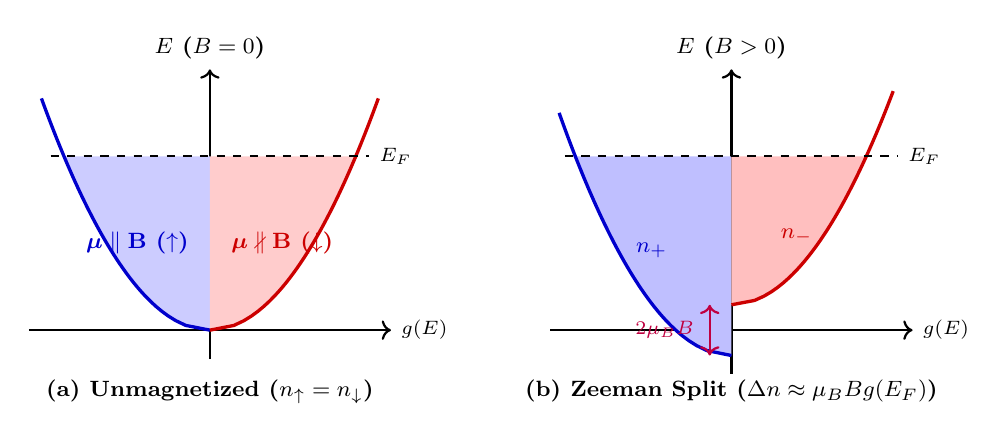
\begin{tikzpicture}[scale=0.92]
  % (a) B = 0
  \begin{scope}[shift={(0,0)}]
    \draw[->, thick] (-2.5,0) -- (2.5,0) node[right, font=\scriptsize] {$g(E)$};
    \draw[->, thick] (0,-0.4) -- (0,3.6) node[above, font=\footnotesize\bfseries] {$E$ ($B = 0$)};
    \fill[blue!20] (0,0) plot[domain=0:2.4, samples=40] ({-1.3*sqrt(\x)}, \x) -- (0,2.4) -- cycle;
    \fill[red!20]  (0,0) plot[domain=0:2.4, samples=40] ({1.3*sqrt(\x)}, \x) -- (0,2.4) -- cycle;
    \draw[blue!80!black, very thick, domain=0:3.2, samples=50] plot ({-1.3*sqrt(\x)}, \x);
    \draw[red!80!black,  very thick, domain=0:3.2, samples=50] plot ({1.3*sqrt(\x)}, \x);
    \draw[dashed, thick] (-2.2,2.4) -- (2.2,2.4) node[right, font=\scriptsize] {$E_F$};
    \node[font=\footnotesize\bfseries, blue!80!black] at (-1.0,1.2) {$\boldsymbol{\mu} \parallel \mathbf{B}$ ($\uparrow$)};
    \node[font=\footnotesize\bfseries, red!80!black]  at (1.0,1.2)  {$\boldsymbol{\mu} \nparallel \mathbf{B}$ ($\downarrow$)};
    \node[below, font=\footnotesize\bfseries] at (0,-0.55) {(a) Unmagnetized ($n_\uparrow = n_\downarrow$)};
  \end{scope}

  % (b) B > 0
  \begin{scope}[shift={(7.2,0)}]
    \draw[->, thick] (-2.5,0) -- (2.5,0) node[right, font=\scriptsize] {$g(E)$};
    \draw[->, thick] (0,-0.6) -- (0,3.6) node[above, font=\footnotesize\bfseries] {$E$ ($B > 0$)};
    \fill[blue!25] (0,-0.35) plot[domain=-0.35:2.4, samples=40] ({-1.3*sqrt(\x+0.35)}, \x) -- (0,2.4) -- cycle;
    \fill[red!25]  (0,0.35)  plot[domain=0.35:2.4, samples=40]  ({1.3*sqrt(\x-0.35)}, \x) -- (0,2.4) -- cycle;
    \draw[blue!80!black, very thick, domain=-0.35:3.0, samples=50] plot ({-1.3*sqrt(\x+0.35)}, \x);
    \draw[red!80!black,  very thick, domain=0.35:3.3, samples=50]  plot ({1.3*sqrt(\x-0.35)}, \x);
    \draw[dashed, thick] (-2.3,2.4) -- (2.3,2.4) node[right, font=\scriptsize] {$E_F$};
    \draw[<->, thick, purple] (-0.3,-0.35) -- (-0.3,0.35) node[midway, left=2pt, font=\scriptsize] {$2\mu_B B$};
    \node[font=\footnotesize\bfseries, blue!80!black] at (-1.1,1.1) {$n_+$};
    \node[font=\footnotesize\bfseries, red!80!black]  at (0.9,1.3)  {$n_-$};
    \node[below, font=\footnotesize\bfseries] at (0,-0.55) {(b) Zeeman Split ($\Delta n \approx \mu_B B g(E_F)$)};
  \end{scope}
\end{tikzpicture}
\caption{Pauli spin paramagnetism of conduction electrons at $T=0$. Applying a field shifts the spin sub-bands by $\mp\mu_BB$, so electrons within $\mu_BB$ of $E_F$ spill into the lower-energy sub-band. The response is small precisely because only this thin shell participates.}
\label{fig:pauli_bands}
\end{figure}

\subsection{Derivation of the Pauli Susceptibility}

Let $g(E)$ be the total density of states (both spins) per unit volume, so each spin direction carries $\frac{1}{2}g(E)$. At $T = 0$ (valid since $T\ll T_F\sim5\times10^{4}\ \mathrm{K}$):
\begin{align}
    n_+ &= \frac{1}{2}\int_{-\mu_BB}^{E_F}g(E+\mu_BB)\,dE
        \approx \frac{1}{2}\int_0^{E_F}g(E)\,dE + \frac{1}{2}\mu_BB\,g(E_F) \notag\\
    n_- &= \frac{1}{2}\int_{+\mu_BB}^{E_F}g(E-\mu_BB)\,dE
        \approx \frac{1}{2}\int_0^{E_F}g(E)\,dE - \frac{1}{2}\mu_BB\,g(E_F)
    \label{eq:paulinplus}
\end{align}
The net excess of aligned moments is $\Delta n = n_+ - n_- = \mu_BB\,g(E_F)$, so
\begin{equation}
    M = \mu_B(n_+ - n_-) = \mu_B^2g(E_F)\,B
    \label{eq:paulimag}
\end{equation}
For a 3D free-electron gas $g(E_F) = \frac{3n}{2E_F} = \frac{3n}{2k_BT_F}$, giving the \textbf{Pauli spin susceptibility}
\begin{equation}
    \boxed{\;\chi_{\mathrm{Pauli}} = \mu_0\mu_B^2g(E_F)
    = \frac{3\mu_0n\mu_B^2}{2k_BT_F}
    = \chi_{\mathrm{Curie}}\cdot\frac{3T}{2T_F}\;}
    \label{eq:pauli}
\end{equation}
Note that $T$ appears only in the ratio $T/T_F$: since $T\ll T_F$, the susceptibility is essentially temperature independent --- the Pauli analogue of the Van Vleck result.

\begin{itemize}[leftmargin=1.6cm]
    \item \textbf{Landau diamagnetism.} In a magnetic field the orbital motion of conduction electrons is quantised into Landau levels, producing a diamagnetic response equal to exactly one-third of the Pauli spin susceptibility (for free electrons with effective mass $m^*$):
    \begin{equation}
        \chi_{\mathrm{Landau}} = -\frac{1}{3}\left(\frac{m_e}{m^*}\right)^2\chi_{\mathrm{Pauli}}
        \;\Longrightarrow\;
        \chi_{\mathrm{total}} = \chi_{\mathrm{Pauli}} + \chi_{\mathrm{Landau}}
        = \frac{2}{3}\chi_{\mathrm{Pauli}}\quad (m^* = m_e)
        \label{eq:landau}
    \end{equation}
\end{itemize}

\begin{takeawaybox}{Why Pauli paramagnetism is so weak}
The Pauli susceptibility is suppressed by a factor of order $T/T_F \sim 10^{-3}$ relative to a Curie spin system of the same moment density. Physically: only the electrons in a shell of width $\mu_BB$ around $E_F$ can respond, whereas in a Curie paramagnet \emph{every} moment responds. This is the same Pauli-exclusion argument that produces the electronic specific heat $\propto T$ --- the same tiny set of electrons does both jobs.
\end{takeawaybox}

\subsection[Adiabatic Demagnetisation (Optional Read)]{Cooling by Adiabatic (Isentropic) Demagnetisation \extratag}
\label{sec:demag}

\begin{enrichmentnote}{Cryogenic Application}
Adiabatic demagnetisation demonstrates how the thermodynamic property $S = S(B/T)$ enables magnetic refrigeration into the millikelvin regime. It is an interesting experimental extension beyond the basic electronic theory syllabus.
\end{enrichmentnote}

For non-interacting spins the magnetic entropy $S(T,B)$ depends only on the population distribution, which is a function solely of $x = \mu_BB/k_BT$, i.e.\ $S = S(B/T)$.

\begin{enumerate}[leftmargin=1.6cm]
    \item \textbf{Step 1 --- isothermal magnetisation at $T_i$.} Apply field $B_i$ while in contact with a helium bath ($T_i\sim1\ \mathrm{K}$). Spins align, the entropy drops from $S(0)$ to $S(B_i/T_i)$, and heat $\Delta Q = T_i\Delta S$ is rejected to the bath.
    \item \textbf{Step 2 --- adiabatic demagnetisation.} Thermally isolate the salt ($\Delta S = 0$) and slowly reduce $B_i\to B_{\mathrm{local}}$, where $B_{\mathrm{local}}\sim10^{-2}\ \mathrm{T}$ is the internal dipolar field. Since $S(B/T) = \text{const}$:
    \begin{equation}
        \frac{B_i}{T_i} = \frac{B_f}{T_f}
        \;\Longrightarrow\;
        \boxed{\;T_f = T_i\frac{B_{\mathrm{local}}}{B_i}\;}
        \label{eq:demag}
    \end{equation}
\end{enumerate}

\begin{pitfallbox}{Why the cooling stops}
The isentropic condition \eqref{eq:demag} assumes the spins are in equilibrium with the applied field. Once $B$ falls to the internal dipolar field $B_{\mathrm{local}}$, the spins are no longer polarised by the applied field and the salt equilibrates with its own internal field. This sets a hard floor at the millikelvin level for electronic spins. Nuclear demagnetisation (e.g.\ of copper) reaches the microkelvin regime because nuclear moments are $\sim10^{-3}$ times smaller and hence the internal fields are far smaller.
\end{pitfallbox}

\clearpage
% =============================================================================
%  CHAPTER 5 --- THE EXCHANGE INTERACTION
% =============================================================================
\section{The Exchange Interaction: Why Spins Order}
\label{ch:exchange}

\subsection{Why Dipole--Dipole Coupling Cannot Explain Ferromagnetism}

\begin{checkpointbox}{Order of magnitude before theory}
Iron has $T_C = 1043\ \mathrm{K}$, so $k_BT_C \approx 0.090\ \mathrm{eV}$ of thermal energy is needed to destroy spin alignment. Estimate the classical dipole--dipole interaction between two neighbouring Bohr magnetons separated by a lattice constant $a\approx2\ \Ang$. How many orders of magnitude short are you?
\end{checkpointbox}

\begin{align}
    U_{\mathrm{dip}} &\approx \frac{\mu_0\mu_B^2}{4\pi a^3}
    = \frac{(10^{-7}\ \mathrm{T\,m/A})(9.27\times10^{-24}\ \mathrm{J/T})^2}{(2\times10^{-10}\ \mathrm{m})^3}
    \approx 1.08\times10^{-24}\ \mathrm{J}
    \approx 6.7\times10^{-6}\ \mathrm{eV}
    \label{eq:dipenergy}\\
    \Longrightarrow\qquad
    T_{\mathrm{dip}} &= \frac{U_{\mathrm{dip}}}{k_B} \approx 0.078\ \mathrm{K}
    \label{eq:dipenergyT}
\end{align}
Since $k_BT_C = 0.090\ \mathrm{eV}$, the dipolar scale is smaller by a factor of $\approx 1.3\times10^{4}$ --- about \textbf{four orders of magnitude}. Direct magnetic dipole coupling is simply far too weak to explain room-temperature ferromagnetism.

\begin{takeawaybox}{The punchline of this section}
Magnetic ordering in iron, cobalt, nickel and the rare earths is driven by the \textbf{electrostatic Coulomb interaction combined with the Pauli Exclusion Principle} --- the \textbf{exchange interaction}. It is an effect of antisymmetry: it exists because electrons are fermions, and it has no classical analogue whatsoever. This is the deep reason the exchange interaction is so much stronger than the dipole interaction, even though it is "only" electrostatic.
\end{takeawaybox}

\subsection{The Two-Electron Toy Model: Heitler--London \texorpdfstring{$\text{H}_2$}{H2}}

Consider two electrons at $\vb{r}_1, \vb{r}_2$ in orbitals $\phi_a, \phi_b$ centred on sites $a$ and $b$. The two-electron Hamiltonian $\mathcal{H} = \mathcal{H}_0 + \frac{e^2}{4\pi\epsilon_0 r_{12}}$ is \emph{completely spin-independent}. However the total wavefunction $\Psi(\vb{r}_1,s_1;\vb{r}_2,s_2) = \psi_{\mathrm{space}}(\vb{r}_1,\vb{r}_2)\chi_{\mathrm{spin}}(s_1,s_2)$ must be \textbf{antisymmetric} under the simultaneous exchange $(1\leftrightarrow 2)$.

\begin{enumerate}[leftmargin=1.6cm]
    \item \textbf{Spin singlet ($S = 0$, antiparallel spins).}
    $\chi_{\mathrm{singlet}} = \frac{1}{\sqrt2}(\uparrow\downarrow - \downarrow\uparrow)$ is \emph{antisymmetric}, so the spatial part must be \textbf{symmetric} (bonding: charge piles up between the nuclei):
    \begin{equation}
        \psi_S(\vb{r}_1,\vb{r}_2) = \frac{1}{\sqrt{2(1+S_{ab}^2)}}\Big[\phi_a(\vb{r}_1)\phi_b(\vb{r}_2) + \phi_b(\vb{r}_1)\phi_a(\vb{r}_2)\Big],
        \qquad E_S = \frac{K+J_{\mathrm{ex}}}{1+S_{ab}^2}\approx K+J_{\mathrm{ex}}
        \label{eq:HeitlerS}
    \end{equation}
    \item \textbf{Spin triplet ($S = 1$, parallel spins).}
    $\chi_{\mathrm{triplet}} = \{\uparrow\uparrow, \frac{1}{\sqrt2}(\uparrow\downarrow+\downarrow\uparrow), \downarrow\downarrow\}$ is \emph{symmetric}, so the spatial part must be \textbf{antisymmetric} (a node at $\vb{r}_1=\vb{r}_2$, creating a \textbf{Fermi hole} that keeps parallel-spin electrons apart):
    \begin{equation}
        \psi_T(\vb{r}_1,\vb{r}_2) = \frac{1}{\sqrt{2(1-S_{ab}^2)}}\Big[\phi_a(\vb{r}_1)\phi_b(\vb{r}_2) - \phi_b(\vb{r}_1)\phi_a(\vb{r}_2)\Big],
        \qquad E_T = \frac{K-J_{\mathrm{ex}}}{1-S_{ab}^2}\approx K-J_{\mathrm{ex}}
        \label{eq:HeitlerT}
    \end{equation}
\end{enumerate}
Here $K$ is the direct Coulomb integral and $J_{\mathrm{ex}}$ the \textbf{exchange integral}. The energy splitting $E_S - E_T = 2J$ depends purely on the total spin $S\in\{0,1\}$.

Using the spin operator identity
\begin{equation}
    \vb{S}_{\mathrm{tot}}^2 = (\vb{s}_1+\vb{s}_2)^2
    = \tfrac34+\tfrac34+2\,\vb{s}_1\cdot\vb{s}_2
    \;\Longrightarrow\;
    \vb{s}_1\cdot\vb{s}_2 = \frac{1}{2}S(S+1)-\frac34
    = \begin{cases}-\tfrac34 & (S=0,\ \text{singlet})\\[2pt] +\tfrac14 & (S=1,\ \text{triplet})\end{cases}
    \label{eq:spinidentity}
\end{equation}
we can write an effective spin Hamiltonian that reproduces both $E_S$ and $E_T$ identically:
\begin{equation}
    \mathcal{H}_{\mathrm{eff}} = \frac{1}{4}(E_S+3E_T) - (E_S-E_T)\,\vb{s}_1\cdot\vb{s}_2
    = \text{const} - 2J\,\vb{s}_1\cdot\vb{s}_2,
    \qquad J \equiv \frac{E_S - E_T}{2}
    \label{eq:Heis2}
\end{equation}

Generalising to a lattice of spins $\vb{S}_i$ gives the \textbf{Heisenberg Hamiltonian}:
\begin{equation}
    \boxed{\;\mathcal{H}_{\mathrm{Heis}} = -2\sum_{\langle i,j\rangle}J_{ij}\,\vb{S}_i\cdot\vb{S}_j
    \;-\; g\mu_B\,\vb{B}\cdot\sum_i\vb{S}_i\;}
    \label{eq:heisenberg}
\end{equation}
where the sum runs over \emph{distinct} nearest-neighbour pairs. The sign of $J$ decides the ordering:
\begin{itemize}[leftmargin=1.6cm]
    \item $J>0 \Rightarrow E_T < E_S \Rightarrow$ \textbf{ferromagnetic} coupling (parallel spins minimise the energy).
    \item $J<0 \Rightarrow E_S < E_T \Rightarrow$ \textbf{antiferromagnetic} coupling (antiparallel spins minimise the energy, as in the covalent $\text{H}_2$ bond).
\end{itemize}

\begin{pitfallbox}{Double-counting in the Heisenberg Hamiltonian}
The prefactor convention matters and is a frequent source of a factor of two. In \eqref{eq:heisenberg} the sum is over \emph{unordered} nearest-neighbour pairs $\langle i,j\rangle$ and the prefactor is $2$. If instead you write $-\sum_{i\neq j}J_{ij}\,\vb{S}_i\cdot\vb{S}_j$ (an \emph{ordered} double sum over $i\neq j$, in which each bond appears twice), the prefactor must be $1$ --- or equivalently you must halve the definition of $J$. Every formula that follows in Chapters 6--8 uses the $\langle i,j\rangle$ convention with prefactor $2$, including $T_C = 2zJS(S+1)/3k_B$.
\end{pitfallbox}

\subsection{Types of Exchange Mechanism in Solids}

\begin{enumerate}[leftmargin=1.6cm]
    \item \textbf{Direct exchange (Bethe--Slater curve).} Direct overlap of neighbouring $d$ orbitals. The sign depends critically on the ratio $r_a/r_{3d}$ (interatomic distance divided by the radius of the $3d$ shell). Small $r_a/r_{3d}$ (Mn, Cr) gives strong overlap $\to$ covalent bonding $\to J<0$ (antiferromagnetic). Intermediate $r_a/r_{3d}$ (Fe, Co, Ni) gives weak overlap, where the intra-atomic Fermi-hole reduction of the Coulomb repulsion wins $\to J>0$ (ferromagnetic).
    \item \textbf{Superexchange.} Indirect coupling of transition-metal cations across an intermediate non-magnetic anion (e.g.\ $\text{Mn}^{2+}$--$\text{O}^{2-}$--$\text{Mn}^{2+}$ in $\text{MnO}$). Usually gives strong antiferromagnetic coupling ($J<0$).
    \item \textbf{RKKY indirect exchange} \extratag\\
    \textbf{(Ruderman--Kittel--Kasuya--Yosida).} In rare-earth metals (Gd, Tb, Dy) the localised $4f$ spins polarise the surrounding sea of conduction electrons with an oscillatory spatial decay:
    \begin{equation}
        J_{\mathrm{RKKY}}(r) \propto \frac{\cos(2k_Fr)}{(2k_Fr)^3}
        \label{eq:rkky}
    \end{equation}
    which can produce ferromagnetic, antiferromagnetic or helical spin order depending on the interatomic spacing.
\end{enumerate}

\begin{figure}[!htbp]
\centering
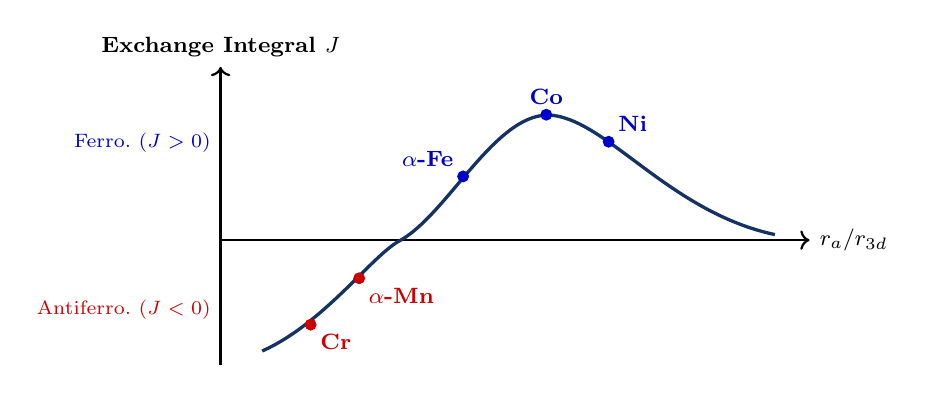
\begin{tikzpicture}[scale=0.88]
  \draw[->, thick] (0,0) -- (8.5,0) node[right, font=\footnotesize\bfseries] {$r_a/r_{3d}$};
  \draw[->, thick] (0,-1.8) -- (0,2.5) node[above, font=\footnotesize\bfseries] {Exchange Integral $J$};
  \node[left, font=\scriptsize, blue!80!black] at (0,1.4) {Ferro.\ ($J>0$)};
  \node[left, font=\scriptsize, red!80!black]  at (0,-1.0) {Antiferro.\ ($J<0$)};

  % Bethe-Slater curve
  \draw[very thick, primary] (0.6,-1.6) .. controls (1.5,-1.2) and (2.2,-0.2) .. (2.6,0)
        .. controls (3.3,0.4) and (4.0,1.9) .. (4.8,1.8)
        .. controls (5.6,1.7) and (6.5,0.4) .. (8.0,0.08);

  % Element points
  \filldraw[red!80!black] (1.3,-1.22) circle (2.2pt) node[below right, font=\footnotesize\bfseries] {Cr};
  \filldraw[red!80!black] (2.0,-0.55) circle (2.2pt) node[below right, font=\footnotesize\bfseries] {$\alpha$-Mn};
  \filldraw[blue!80!black] (3.5,0.92) circle (2.2pt) node[above left, font=\footnotesize\bfseries] {$\alpha$-Fe};
  \filldraw[blue!80!black] (4.7,1.81) circle (2.2pt) node[above, font=\footnotesize\bfseries] {Co};
  \filldraw[blue!80!black] (5.6,1.42) circle (2.2pt) node[above right, font=\footnotesize\bfseries] {Ni};
\end{tikzpicture}
\caption{The Bethe--Slater curve: the sign and magnitude of the direct exchange integral $J$ as a function of the ratio $r_a/r_{3d}$ (interatomic distance divided by the radius of the $3d$ shell) for $3d$ transition metals. Chromium and $\alpha$-Mn sit in the antiferromagnetic region; Fe, Co and Ni sit in the ferromagnetic region.}
\label{fig:bethe_slater}
\end{figure}

% =============================================================================
%  CHAPTER 6 --- FERROMAGNETISM
% =============================================================================
\section{Ferromagnetism and Weiss Molecular Field Theory}
\label{ch:ferro}

\subsection{From the Heisenberg Hamiltonian to the Weiss Exchange Field}

Consider site $i$ in \eqref{eq:heisenberg}, interacting with $z$ nearest neighbours through $J$:
\begin{equation}
    \mathcal{H}_i = -2J\,\vb{S}_i\cdot\sum_{\delta=1}^{z}\vb{S}_{i+\delta} - g\mu_B\,\vb{S}_i\cdot\vb{B}_a
    \label{eq:siteH}
\end{equation}
In the \textbf{mean-field (Weiss molecular field) approximation} we neglect correlated fluctuations $(\vb{S}_i-\langle\vb{S}\rangle)\cdot(\vb{S}_j-\langle\vb{S}\rangle)$ and replace the neighbour spins by their thermal average $\langle\vb{S}_{i+\delta}\rangle = \langle\vb{S}\rangle$. With $\vb{M} = -Ng\mu_B\langle\vb{S}\rangle$:
\begin{equation}
    \mathcal{H}_i^{\mathrm{MF}} = -g\mu_B\,\vb{S}_i\cdot\left(\vb{B}_a + \vb{B}_E\right)
    \;\Longrightarrow\;
    \vb{B}_E = -\frac{2zJ}{g\mu_B}\langle\vb{S}\rangle
    = \frac{2zJ}{Ng^2\mu_B^2}\,\vb{M}
    \equiv \lambda\vb{M}
    \label{eq:weissfield}
\end{equation}
so that the effective field experienced by every spin is
\begin{equation}
    \boxed{\;\vb{B}_{\mathrm{eff}} = \vb{B}_a + \lambda\vb{M},
    \qquad \lambda = \frac{2zJ}{Ng^2\mu_B^2}\;}
    \label{eq:beff}
\end{equation}

\begin{examplebox}{The exchange field in iron}{ex:Bfield}
Take $T_C \approx 1000\ \mathrm{K}$ for iron. The mean-field relation $T_C = \lambda C$ (derived below) gives $\lambda = T_C/C$, and with $C = \frac{\mu_0Ng^2\mu_B^2S(S+1)}{3k_B}$ the exchange field at saturation works out to
\[
B_E = \lambda M_s \approx \frac{2zJS}{g\mu_B} \sim 10^{3}\ \mathrm{T}\quad (10^{7}\ \mathrm{G}).
\]
This is roughly $10^{4}$ times the strongest steady laboratory field ever produced. \emph{Interpretation:} the exchange field is not an applied field at all --- it is generated spontaneously by the neighbouring spins themselves, and it is enormous. Any hand-waving picture in which "the magnetisation aligns the spins" needs this number attached to it to be credible.
\end{examplebox}

\subsection{Paramagnetic Regime \texorpdfstring{($T>T_C$)}{(T > TC)}: the Curie--Weiss Law}

Above the critical temperature $T_C$ the spontaneous magnetisation vanishes and a small applied field induces a small magnetisation. \emph{Convention for this chapter and the next: we work in CGS, as Kittel does.} The Curie law in the field variable is $M = \frac{C}{T}H_{\mathrm{eff}}$ with $C = \frac{Ng^2\mu_B^2S(S+1)}{3k_B}$ (CGS). Replacing $H \to H_a + \lambda M$:
\begin{equation}
    MT = C(H_a + \lambda M)
    \;\Longrightarrow\;
    M(T - C\lambda) = CH_a
    \;\Longrightarrow\;
    \boxed{\;\chi = \frac{M}{H_a} = \frac{C}{T - T_C}\;},
    \qquad T_C = \lambda C
    \label{eq:curieweiss}
\end{equation}
the \textbf{Curie--Weiss law}, with the ferromagnetic Curie temperature directly related to the microscopic exchange integral:
\begin{equation}
    \boxed{\;T_C = \lambda C
    = \left(\frac{2zJ}{Ng^2\mu_B^2}\right)\left(\frac{Ng^2\mu_B^2S(S+1)}{3k_B}\right)
    = \frac{2zJS(S+1)}{3k_B}\;}
    \label{eq:Tc}
\end{equation}

\begin{methodbox}{Recipe: the Curie--Weiss law, in CGS and in SI}
\begin{itemize}[leftmargin=1.4cm, itemsep=1pt]
    \item \textbf{CGS:} $\chi = M/H$ and $\chi = C/(T-T_C)$ with $T_C = \lambda C$, $\lambda = 2zJ/(Ng^2\mu_B^2)$ and $C = Ng^2\mu_B^2S(S+1)/3k_B$.
    \item \textbf{SI:} $\chi = \mu_0M/B$ and $\chi = C/(T-T_C)$ with $C = \mu_0Ng^2\mu_B^2S(S+1)/3k_B$; the molecular-field coefficient multiplies $\vb{M}$ in \emph{tesla}, $\lambda = 2zJ/(Ng^2\mu_B^2)$, so $T_C = \lambda C/\mu_0$.
    \item Both routes give the same physical result, $T_C = 2zJS(S+1)/3k_B$.
    \item \textbf{Sanity check:} $J>0$ (ferromagnetic) $\Rightarrow T_C>0$; $J<0$ (antiferromagnetic) $\Rightarrow$ the same algebra gives a \emph{negative} intercept, which is the origin of the "negative Weiss temperature" of antiferromagnets (Chapter 8).
\end{itemize}
\end{methodbox}

\subsection{Ferromagnetic Regime \texorpdfstring{($T<T_C$)}{(T < TC)}: Spontaneous Magnetisation}

Set $\vb{B}_a = 0$, so $\vb{B}_{\mathrm{eff}} = \lambda\vb{M}$. Substituting into the exact Brillouin equation:
\begin{equation}
    M(T) = M_0\,B_S(x),
    \qquad M_0 = Ng\mu_BS,
    \qquad x = \frac{g\mu_BS(\lambda M)}{k_BT}
    \label{eq:Mselfcons}
\end{equation}
Expressing $\lambda = \frac{3k_BT_C}{Ng^2\mu_B^2S(S+1)}$ and eliminating $M$ in favour of $x$:
\begin{equation}
    \boxed{\;\frac{M(T)}{M_0} = B_S(x) = \left(\frac{S+1}{3S}\right)\left(\frac{T}{T_C}\right)x\;}
    \label{eq:selfcons}
\end{equation}
For the simplest case $S = 1/2$ ($g = 2$), $B_{1/2}(x) = \tanh x$ and $\frac{S+1}{3S} = 1$, so
\begin{equation}
    \boxed{\;m \equiv \frac{M(T)}{M_0} = \tanh\!\left(\frac{T_C}{T}\,m\right)
    \quad\Longleftrightarrow\quad
    \tanh x = \left(\frac{T}{T_C}\right)x\;}
    \label{eq:tanhselfcons}
\end{equation}

\begin{figure}[!htbp]
\centering
\includegraphics[width=\textwidth]{figures/fig_weiss.pdf}
\caption{The mean-field self-consistency equation. \textbf{(a)} Graphical solution of $\tanh x = (T/T_C)x$: for $T>T_C$ the line is steeper than $\tanh$ and the only solution is $x=0$; for $T<T_C$ a non-trivial solution $x^*>0$ exists, and that solution \emph{is} the spontaneous magnetisation. \textbf{(b)} The resulting universal magnetisation curve $M(T)/M(0)$ versus $T/T_C$, showing the square-root onset at $T_C$.}
\label{fig:weiss}
\end{figure}

\paragraph{Asymptotic behaviour near $T\to T_C^-$ (critical exponent $\beta = 1/2$).}
Near $T_C$, $m\ll1$. Expanding $\tanh u\approx u - \frac{1}{3}u^3$:
\begin{equation}
    m \approx \left(\frac{T_C}{T}\right)m - \frac{1}{3}\left(\frac{T_C}{T}\right)^3m^3
    \;\Longrightarrow\;
    \frac{1}{3}\left(\frac{T_C}{T}\right)^3m^2 = \frac{T_C-T}{T}
    \;\Longrightarrow\;
    \boxed{\;\frac{M(T)}{M_0}\approx\sqrt{3}\left(1-\frac{T}{T_C}\right)^{1/2}\;}
    \label{eq:beta}
\end{equation}
so the mean-field critical exponent is $\beta = 1/2$.

\paragraph{Asymptotic behaviour near $T\to 0$: mean-field failure.}
As $T\to0$, $\tanh x \approx 1 - 2e^{-2x}$, so mean-field theory predicts an exponential approach $M(T)/M_0 \approx 1 - 2\exp(-2T_C/T)$. \textbf{Experiment instead shows a power law $\Delta M\propto T^{3/2}$.} The reason is that mean-field theory assumes a single spin must flip completely against the entire exchange field ($\Delta E = 2zJS$), ignoring collective long-wavelength \textbf{spin waves} --- the subject of the next section.

\begin{checkpointbox}{Why must the mean-field $T\to0$ law be wrong?}
Mean field gives $1 - M(T)/M_0 \propto e^{-2T_C/T}$; experiment gives $\propto T^{3/2}$. Which of the two decays \emph{faster} as $T\to0$, and what does that tell you about which description has more "states" available to absorb thermal energy?
\end{checkpointbox}

\subsection[Band Ferromagnetism \& Stoner Criterion (Optional Read)]{Band (Itinerant) Ferromagnetism and the Stoner Criterion \extratag}
\label{sec:stoner}

\begin{enrichmentnote}{Itinerant Magnetism}
While the Heisenberg and Weiss models treat localised atomic moments, $3d$ electrons in metals (Fe, Co, Ni) are delocalised in energy bands with non-integer Bohr magneton numbers. The Stoner criterion $I\cdot g(E_F) > 1$ explains why spontaneous band splitting occurs in Fe, Co and Ni but not Cu. It is an optional enrichment topic beyond the localized Heisenberg syllabus.
\end{enrichmentnote}

In the $3d$ transition metals (Fe, Co, Ni) the $3d$ electrons are itinerant --- delocalised in narrow energy bands --- and carry non-integer magnetic moments per atom (Ni: $0.60\ \mu_B$, Co: $1.72\ \mu_B$, Fe: $2.22\ \mu_B$). Suppose we spontaneously transfer $\delta n$ electrons from the spin-down band to the spin-up band at $E_F$:
\begin{itemize}[leftmargin=1.6cm]
    \item \textbf{Kinetic energy cost:} $\Delta E_{\mathrm{kin}} = +\frac{1}{2}\frac{(\delta n)^2}{g(E_F)/2} = \frac{(\delta n)^2}{g(E_F)}$
    \item \textbf{Exchange energy gain:} $\Delta E_{\mathrm{ex}} = -\frac{1}{2}I(\delta n)^2$, with $I$ the Stoner exchange parameter.
\end{itemize}
Spontaneous band splitting ($\Delta E_{\mathrm{tot}} < 0$) occurs when the \textbf{Stoner criterion} is satisfied:
\begin{equation}
    \boxed{\;I\cdot g(E_F) > 1\;}
    \label{eq:stoner}
\end{equation}
This explains why Fe, Co and Ni --- where $E_F$ sits inside a high-density $3d$ peak --- are ferromagnetic, whereas Cu --- where $E_F$ lies in the low-density $4s$ band above the filled $3d$ band --- is not. Pd and Pt are the interesting borderline cases: "nearly ferromagnetic" Stoner-enhanced paramagnets.

% =============================================================================
%  CHAPTER 7 --- MAGNONS, DOMAINS, HYSTERESIS
% =============================================================================
\section[Magnons, Domains and Hysteresis (Optional Extension)]{Magnons, Domains and Hysteresis \extratag}
\label{ch:magnons}

\begin{enrichmentnote}{Collective Excitations and Microstructure}
The core PH7302 syllabus focuses on exchange and mean-field ordering. This chapter explores microscopic collective excitations (magnons / spin waves and Bloch's $T^{3/2}$ law) as well as macroscopic domain microstructures (Bloch walls, demagnetising fields and hysteresis). These sections provide essential physical depth and preparation for competitive examinations (NET/GATE), but detailed mathematical derivations here go beyond the compulsory semester syllabus.
\end{enrichmentnote}

\subsection[Ferromagnetic Magnons and Bloch T3/2 Law (Optional Read)]{Ferromagnetic Magnons and Bloch's \texorpdfstring{$T^{3/2}$}{T3/2} Law \extratag}

In the ground state of a ferromagnet all spins are parallel ($U_0 = -2NJS^2$ for a 1D chain). Reversing a single spin costs $\Delta E = 8JS^2$. A far lower-energy excitation is obtained by tilting all spins slightly and letting them precess on cones with a constant phase advance $ka$ between neighbours --- a \textbf{spin wave}, quantised as a boson called a \textbf{magnon}.

\begin{enumerate}[leftmargin=1.6cm]
    \item \textbf{Equations of motion.} Using
    \begin{equation}
        \frac{d\vb{S}_p}{dt} = \frac{1}{\hbar}\left(\vb{S}_p\times\text{torque}\right)
        = -\frac{2J}{\hbar}\vb{S}_p\times\left(\vb{S}_{p-1}+\vb{S}_{p+1}\right)
        \label{eq:magnoneom}
    \end{equation}
    and linearising ($S_p^z\approx S$, $S_p^x,S_p^y\ll S$) for a plane wave $\propto e^{i(pka-\omega t)}$, one obtains the \textbf{ferromagnetic magnon dispersion}
    \begin{equation}
        \boxed{\;\hbar\omega_k = 4JS(1-\cos ka)
        \xrightarrow{ka\ll1} 2JSa^2k^2 \equiv Dk^2
        \quad (\text{3D cubic: } \hbar\omega_k = 2JSa^2k^2)\;}
        \label{eq:magnondisp}
    \end{equation}
    Note the \textbf{quadratic dispersion} ($\omega\propto k^2$) at long wavelengths --- the hallmark of a ferromagnet.
    \item \textbf{Bloch's $T^{3/2}$ law.} Each thermally excited magnon reduces the total spin projection by one ($\Delta M = g\mu_B\sum_k n_k$), and magnons obey Bose--Einstein statistics with zero chemical potential:
    \begin{equation}
        \sum_k n_k = \int\frac{d^3k}{(2\pi)^3}\frac{1}{e^{\hbar\omega_k/k_BT}-1}
        = \frac{1}{2\pi^2}\int_0^\infty\frac{k^2\,dk}{e^{Dk^2/k_BT}-1}
        \propto \left(\frac{k_BT}{D}\right)^{3/2}
        \label{eq:magnonpop}
    \end{equation}
    Evaluating the resulting Riemann zeta integral gives \textbf{Bloch's $T^{3/2}$ law} for both the fractional magnetisation drop and the magnon heat capacity:
    \begin{equation}
        \boxed{\;\frac{\Delta M(T)}{M(0)} = \frac{M(0)-M(T)}{M(0)}
        = \frac{0.0587}{SQ}\left(\frac{k_BT}{2JS}\right)^{3/2}\propto T^{3/2},
        \qquad C_{\mathrm{mag}}\propto T^{3/2}\;}
        \label{eq:bloch}
    \end{equation}
    where $Q = 1, 2, 4$ for simple cubic, bcc and fcc lattices respectively.
\end{enumerate}

\begin{examplebox}{Deriving the two magnon heat-capacity laws}{ex:magnonC}
The two cases differ through the dispersion relation, and the evaluation is carried out via standard Bose--Einstein integration.

\medskip
\textit{Ferromagnet ($\hbar\omega = Dk^2$).} The magnon energy per unit volume is
\[
U = \frac{1}{2\pi^2}\int_0^\infty k^2\,dk\,\frac{Dk^2}{e^{Dk^2/k_BT}-1}.
\]
Substituting $u = Dk^2/k_BT$, we have $k = (k_BT/D)^{1/2}u^{1/2}$, $k^2dk = \tfrac12(k_BT/D)^{3/2}u^{1/2}du$, and the numerator is $Dk^2 = (k_BT)u$. The total energy density becomes
\[
U = \frac{1}{4\pi^2}\left(\frac{k_BT}{D}\right)^{3/2}(k_BT)\int_0^\infty \frac{u^{3/2}}{e^u-1}du
= \frac{(k_BT)^{5/2}}{4\pi^2 D^{3/2}}\,\Gamma(5/2)\zeta(5/2).
\]
Using $\Gamma(5/2)\zeta(5/2) = \frac{3\sqrt{\pi}}{4}\times 1.34149 \approx 1.7833$, we find $U \approx 0.04517\,\frac{(k_BT)^{5/2}}{D^{3/2}}$. Differentiating with respect to temperature gives the heat capacity:
\[
\boxed{C_{\mathrm{mag,FM}} = \frac{\partial U}{\partial T} = \frac{5}{2}\frac{k_B(k_BT)^{3/2}}{4\pi^2 D^{3/2}}\Gamma(5/2)\zeta(5/2) \approx 0.1129\,k_B\left(\frac{k_BT}{D}\right)^{3/2} \propto T^{3/2}}.
\]
Notice that the dimensions are completely consistent: $[k_BT/D] = \mathrm{m^{-2}}$, so $[k_B(k_BT/D)^{3/2}] = \mathrm{J/(K\cdot m^3)}$ (heat capacity per unit volume).

\medskip
\textit{Antiferromagnet ($\hbar\omega = ck$, $c = 4|J|Sa$).}
\[
U = \frac{1}{2\pi^2}\int_0^\infty k^2\,dk\,\frac{ck}{e^{ck/k_BT}-1}
= \frac{c}{2\pi^2}\left(\frac{k_BT}{c}\right)^4\int_0^\infty\frac{u^3}{e^u-1}du,
\]
and since $\int_0^\infty\frac{u^3}{e^u-1}du = \frac{\pi^4}{15}$:
\[
U = \frac{\pi^2}{30}\frac{(k_BT)^4}{c^3}
\;\Longrightarrow\;
\boxed{C_{\mathrm{mag,AFM}} = \frac{2\pi^2}{15}k_B\left(\frac{k_BT}{4|J|Sa}\right)^3 \propto T^3}.
\]

\medskip
\textit{Rule of thumb.} In $d$ dimensions a dispersion $\omega\propto k^s$ gives $C_{\mathrm{mag}}\propto T^{d/s}$: quadratic ($s=2$) in 3D gives $T^{3/2}$; linear ($s=1$) in 3D gives $T^3$.
\end{examplebox}

\begin{figure}[!htbp]
\centering
\includegraphics[width=\textwidth]{figures/fig_magnon.pdf}
\caption{Magnon physics. \textbf{(a)} The ferromagnetic branch is quadratic in $k$ and the antiferromagnetic branch is linear --- the same contrast that appears in the heat-capacity exponents. \textbf{(b)} Bloch's $T^{3/2}$ law for the fractional magnetisation drop, for the three cubic lattice types ($Q = 1,2,4$).}
\label{fig:magnon}
\end{figure}

\subsection[Domains, Bloch Walls and Hysteresis (Optional Read)]{Domains, Bloch Walls and Hysteresis \extratag}

Why is a piece of iron at room temperature not a strong permanent magnet? Because a uniformly magnetised block creates a huge external stray field $\vb{B}_{\mathrm{stray}}$ with magnetostatic energy $\int\frac{B^2}{2\mu_0}\,dV$. To minimise this energy the crystal subdivides into macroscopic \textbf{Weiss domains} with closure flux patterns.

\paragraph{Thickness and energy of a Bloch wall.}
The boundary between two antiparallel domains (a $180^\circ$ rotation) is a \textbf{Bloch wall}. Why does the spin not reverse abruptly in a single atomic step?
\begin{itemize}[leftmargin=1.6cm]
    \item Between two spins tilted by a small angle $\phi$ the exchange cost is $w_{\mathrm{ex}} = -2JS^2\cos\phi - (-2JS^2)\approx JS^2\phi^2$.
    \item If a total rotation of $\pi$ radians is spread over $N$ atomic planes then $\phi = \pi/N$, and the total exchange energy of a line of $N$ spins is
    \begin{equation}
        E_{\mathrm{ex,line}} = N\cdot JS^2\left(\frac{\pi}{N}\right)^2 = \frac{\pi^2JS^2}{N}
        \label{eq:wallex}
    \end{equation}
    so exchange energy alone favours $N\to\infty$ --- an infinitely thick wall.
    \item What stops the wall from growing without limit is the \textbf{magnetocrystalline anisotropy energy $K$} (arising from spin--orbit coupling, which locks spins along easy crystallographic axes such as $[100]$ in Fe or the $c$-axis in Co). Spins inside the wall point along hard directions, costing anisotropy energy per unit area $\sigma_{\mathrm{anis}}\approx KNa$.
    \item Minimising the total wall energy per unit area $\sigma_{\mathrm{wall}} = \sigma_{\mathrm{ex}} + \sigma_{\mathrm{anis}}$ with respect to $N$:
    \begin{equation}
        \sigma_{\mathrm{wall}}(N) = \frac{\pi^2JS^2}{Na^2} + KNa,
        \qquad \frac{\partial\sigma_{\mathrm{wall}}}{\partial N} = 0
        \label{eq:wallwidth}
    \end{equation}
    \begin{equation}
        \boxed{\;N = \pi\sqrt{\frac{JS^2}{Ka^3}} \sim 300\ \text{planes}
        \quad (\delta \sim 100\ \mathrm{nm})\;}
    \end{equation}
\end{itemize}

\begin{figure}[!htbp]
\centering
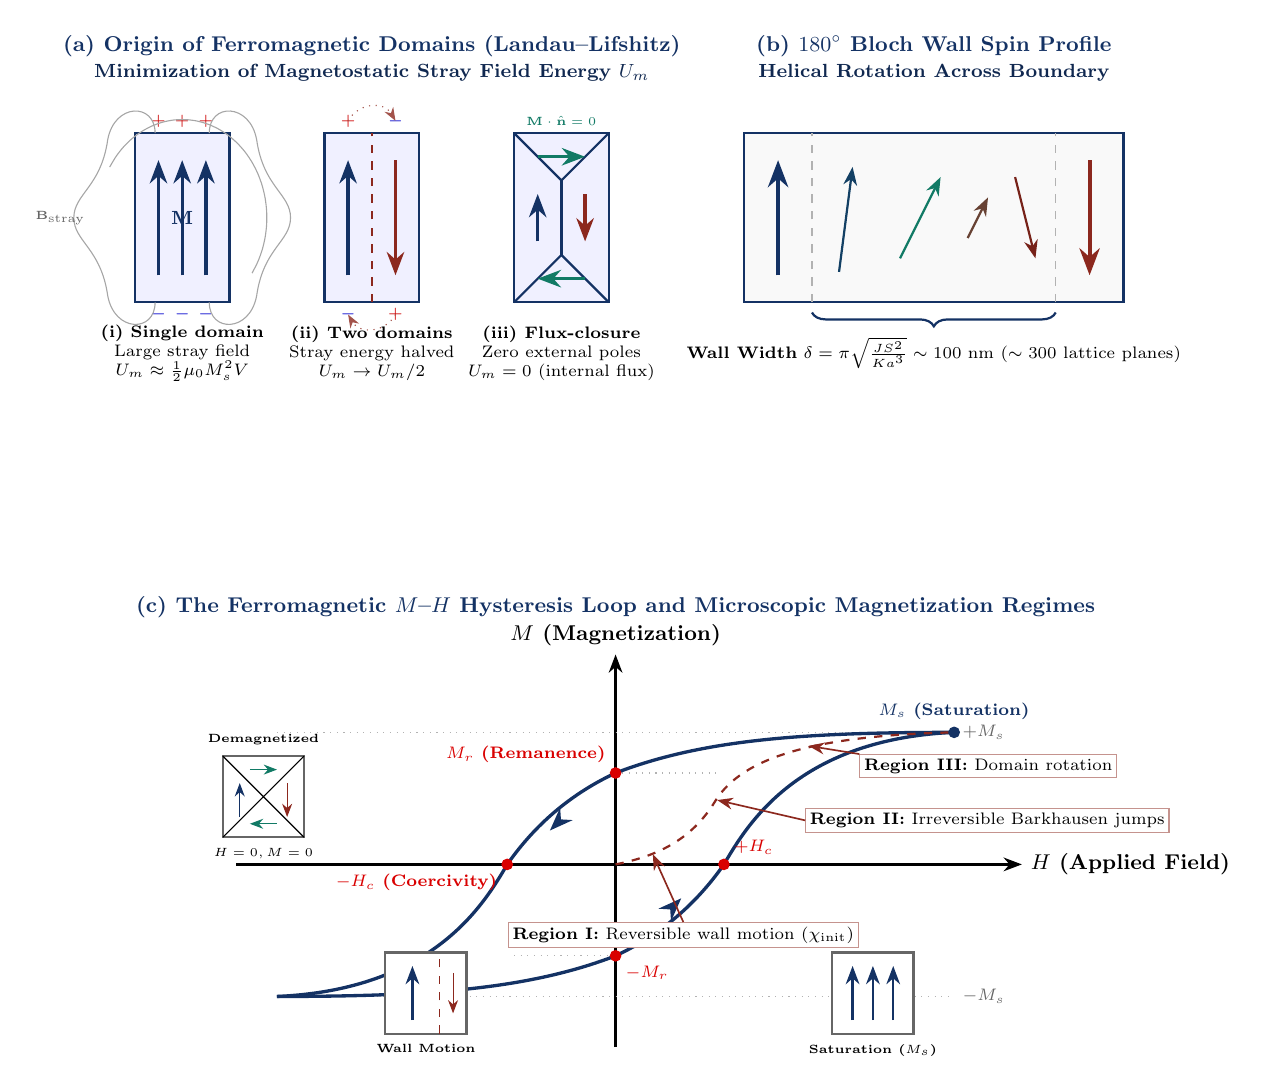
\begin{tikzpicture}[>=Stealth, scale=0.86, every node/.style={transform shape}]

  % -------------------------------------------------------------------------
  % TOP ROW: Panel (a) and Panel (b)
  % -------------------------------------------------------------------------
  \begin{scope}[shift={(0, 7.2)}]

    % Section Title for Panel (a)
    \node[align=center, font=\small\bfseries, text=primary] at (3.9, 4.1) 
      {(a) Origin of Ferromagnetic Domains (Landau--Lifshitz)\\ \color{primary!80!black}\footnotesize Minimization of Magnetostatic Stray Field Energy $U_m$};

    % Sub-panel (i): Single Large Domain
    \draw[thick, fill=blue!6, draw=primary] (0.4, 0.5) rectangle (1.8, 3.0);
    \foreach \x in {0.75, 1.1, 1.45} {
      \draw[->, very thick, primary] (\x, 0.9) -- (\x, 2.6);
    }
    \node[font=\footnotesize\bfseries, primary] at (1.1, 1.75) {$\mathbf{M}$};
    % Surface magnetic poles
    \node[font=\scriptsize\bfseries, red!80!black] at (0.75, 3.18) {$+$};
    \node[font=\scriptsize\bfseries, red!80!black] at (1.1, 3.18) {$+$};
    \node[font=\scriptsize\bfseries, red!80!black] at (1.45, 3.18) {$+$};
    \node[font=\scriptsize\bfseries, blue!80!black] at (0.75, 0.32) {$-$};
    \node[font=\scriptsize\bfseries, blue!80!black] at (1.1, 0.32) {$-$};
    \node[font=\scriptsize\bfseries, blue!80!black] at (1.45, 0.32) {$-$};
    % Stray field lines (schematic dipole loops)
    \draw[domain=-0.6:2.6, smooth, variable=\t, gray!70, thin] 
      plot ({1.1 + 1.25*cos(\t r)}, {1.75 + 1.45*sin(\t r)});
    \draw[gray!70, thin] (0.7, 3.0) .. controls (0.7, 3.45) and (0.1, 3.45) .. (0.0, 2.9)
                                   .. controls (-0.1, 2.2) and (-0.5, 2.1) .. (-0.5, 1.75)
                                   .. controls (-0.5, 1.4) and (-0.1, 1.3) .. (0.0, 0.6)
                                   .. controls (0.1, 0.05) and (0.7, 0.05) .. (0.7, 0.5);
    \draw[gray!70, thin] (1.5, 3.0) .. controls (1.5, 3.45) and (2.1, 3.45) .. (2.2, 2.9)
                                   .. controls (2.3, 2.2) and (2.7, 2.1) .. (2.7, 1.75)
                                   .. controls (2.7, 1.4) and (2.3, 1.3) .. (2.2, 0.6)
                                   .. controls (2.1, 0.05) and (1.5, 0.05) .. (1.5, 0.5);
    \node[font=\tiny, gray!80!black] at (-0.7, 1.75) {$\mathbf{B}_{\text{stray}}$};
    \node[align=center, font=\scriptsize] at (1.1, -0.25) 
      {\textbf{(i) Single domain}\\ Large stray field\\ $U_m \approx \frac{1}{2}\mu_0 M_s^2 V$};

    % Sub-panel (ii): Two Antiparallel Domains
    \draw[thick, fill=blue!6, draw=primary] (3.2, 0.5) rectangle (4.6, 3.0);
    \draw[dashed, thick, secondary] (3.9, 0.5) -- (3.9, 3.0);
    \draw[->, very thick, primary] (3.55, 0.9) -- (3.55, 2.6);
    \draw[->, very thick, secondary] (4.25, 2.6) -- (4.25, 0.9);
    \node[font=\scriptsize\bfseries, red!80!black] at (3.55, 3.18) {$+$};
    \node[font=\scriptsize\bfseries, blue!80!black] at (4.25, 3.18) {$-$};
    \node[font=\scriptsize\bfseries, blue!80!black] at (3.55, 0.32) {$-$};
    \node[font=\scriptsize\bfseries, red!80!black] at (4.25, 0.32) {$+$};
    % Local stray field loop between adjacent opposite poles
    \draw[->, dotted, thin, secondary!80] (3.55, 3.18) to[out=60, in=120, looseness=1.2] (4.25, 3.18);
    \draw[->, dotted, thin, secondary!80] (4.25, 0.32) to[out=-120, in=-60, looseness=1.2] (3.55, 0.32);
    \node[align=center, font=\scriptsize] at (3.9, -0.25) 
      {\textbf{(ii) Two domains}\\ Stray energy halved\\ $U_m \to U_m/2$};

    % Sub-panel (iii): Closure Domains (Landau--Lifshitz Structure)
    \draw[thick, fill=blue!6, draw=primary] (6.0, 0.5) rectangle (7.4, 3.0);
    \draw[thick, primary] (6.0, 3.0) -- (6.7, 2.3) -- (7.4, 3.0);
    \draw[thick, primary] (6.0, 0.5) -- (6.7, 1.2) -- (7.4, 0.5);
    \draw[thick, primary] (6.7, 1.2) -- (6.7, 2.3);
    % Arrows in 4 domains
    \draw[->, very thick, primary] (6.35, 1.4) -- (6.35, 2.1);
    \draw[->, very thick, secondary] (7.05, 2.1) -- (7.05, 1.4);
    \draw[->, very thick, tealcol] (6.35, 2.65) -- (7.05, 2.65);
    \draw[->, very thick, tealcol] (7.05, 0.85) -- (6.35, 0.85);
    \node[font=\tiny\bfseries, tealcol] at (6.7, 3.18) {$\mathbf{M} \cdot \hat{\mathbf{n}} = 0$};
    \node[align=center, font=\scriptsize] at (6.7, -0.25) 
      {\textbf{(iii) Flux-closure}\\ Zero external poles\\ $U_m = 0$ (internal flux)};

    % Section Title for Panel (b)
    \node[align=center, font=\small\bfseries, text=primary] at (12.2, 4.1) 
      {(b) $180^\circ$ Bloch Wall Spin Profile\\ \color{primary!80!black}\footnotesize Helical Rotation Across Boundary};

    % Panel (b): 180-degree Bloch Wall Transition
    \draw[thick, fill=gray!5, draw=primary] (9.4, 0.5) rectangle (15.0, 3.0);
    \draw[dashed, gray!60] (10.4, 0.5) -- (10.4, 3.0);
    \draw[dashed, gray!60] (14.0, 0.5) -- (14.0, 3.0);

    % Domain 1 spin (Up)
    \draw[->, line width=1.5pt, primary] (9.9, 0.9) -- (9.9, 2.6);
    
    % Spins inside the Bloch wall rotating out of plane (helical)
    \draw[->, thick, primary!80!tealcol] (10.8, 0.95) -- (11.0, 2.5);
    \draw[->, thick, tealcol] (11.7, 1.15) -- (12.3, 2.35);
    \draw[->, thick, secondary!70!tealcol] (12.7, 1.45) -- (13.0, 2.05);
    \draw[->, thick, secondary!85!black] (13.4, 2.35) -- (13.7, 1.15);

    % Domain 2 spin (Down)
    \draw[->, line width=1.5pt, secondary] (14.5, 2.6) -- (14.5, 0.9);

    % Bloch Wall Width Brace
    \draw[decorate, decoration={brace, amplitude=5pt, mirror}, thick, primary]
      (10.4, 0.35) -- (14.0, 0.35);
    \node[below=7pt, font=\scriptsize, align=center] at (12.2, 0.35) 
      {\textbf{Wall Width} $\delta = \pi \sqrt{\frac{JS^2}{Ka^3}} \sim 100\text{ nm}$ ($\sim 300\text{ lattice planes}$)};

  \end{scope}

  % -------------------------------------------------------------------------
  % BOTTOM ROW: Panel (c) Ferromagnetic M-H Hysteresis Loop
  % -------------------------------------------------------------------------
  \begin{scope}[shift={(7.5, -0.6)}]

    % Title
    \node[align=center, font=\small\bfseries, text=primary] at (0, 3.8) 
      {(c) The Ferromagnetic $M$--$H$ Hysteresis Loop and Microscopic Magnetization Regimes};

    % Axes
    \draw[->, >=Stealth, thick] (-5.6, 0) -- (6.0, 0) node[right, font=\small\bfseries] {$H$ (Applied Field)};
    \draw[->, >=Stealth, thick] (0, -2.7) -- (0, 3.1) node[above, font=\small\bfseries] {$M$ (Magnetization)};

    % Grid / Reference Lines
    \draw[dotted, gray!60] (-5.0, 1.95) -- (5.0, 1.95);
    \draw[dotted, gray!60] (-5.0, -1.95) -- (5.0, -1.95);
    \draw[dotted, gray!60] (0, 1.35) -- (1.5, 1.35);
    \draw[dotted, gray!60] (-1.5, -1.35) -- (0, -1.35);
    \node[right, font=\scriptsize, gray!80!black] at (5.0, 1.95) {$+M_s$};
    \node[right, font=\scriptsize, gray!80!black] at (5.0, -1.95) {$-M_s$};

    % Upper Branch (Descending from Saturation)
    \draw[very thick, primary] 
      (5.0, 1.95) .. controls (2.8, 1.95) and (1.3, 1.85) .. (0, 1.35)
                  .. controls (-0.75, 1.0) and (-1.25, 0.5) .. (-1.6, 0)
                  .. controls (-1.95, -0.6) and (-2.7, -1.85) .. (-5.0, -1.95);

    % Lower Branch (Ascending towards Saturation)
    \draw[very thick, primary] 
      (-5.0, -1.95) .. controls (-2.8, -1.95) and (-1.3, -1.85) .. (0, -1.35)
                    .. controls (0.75, -1.0) and (1.25, -0.5) .. (1.6, 0)
                    .. controls (1.95, 0.6) and (2.7, 1.85) .. (5.0, 1.95);

    % Virgin (Initial) Magnetization Curve: starts at (0,0)
    \draw[thick, dashed, secondary] 
      (0, 0) .. controls (0.6, 0.12) and (1.1, 0.35) .. (1.45, 0.9)
             .. controls (1.8, 1.5) and (2.7, 1.9) .. (5.0, 1.95);

    % Directional Arrows along branches
    \draw[->, very thick, primary] (-0.85, 0.62) -- (-0.97, 0.50);
    \draw[->, very thick, primary] (0.85, -0.62) -- (0.97, -0.50);

    % Key Parameter Dots (EXACTLY ON CURVES)
    \filldraw[red!85!black] (0, 1.35) circle (2.2pt) node[above left=1pt, font=\scriptsize\bfseries] {$M_r$ (Remanence)};
    \filldraw[red!85!black] (0, -1.35) circle (2.2pt) node[below right=1pt, font=\scriptsize\bfseries] {$-M_r$};
    \filldraw[red!85!black] (-1.6, 0) circle (2.2pt) node[below left=1pt, font=\scriptsize\bfseries] {$-H_c$ (Coercivity)};
    \filldraw[red!85!black] (1.6, 0) circle (2.2pt) node[above right=1pt, font=\scriptsize\bfseries] {$+H_c$};
    \filldraw[primary] (5.0, 1.95) circle (2.2pt) node[above=2pt, font=\scriptsize\bfseries] {$M_s$ (Saturation)};

    % Virgin Curve Regimes: Clean Callouts pointing directly to the curve features
    % Region I: Reversible toe
    \node[below, font=\scriptsize, align=center, fill=white, inner sep=1.8pt, draw=secondary!50] (reg1) at (1.0, -0.85) 
      {\textbf{Region I:} Reversible wall motion ($\chi_{\text{init}}$)};
    \draw[->, secondary, semithick] (reg1.north) -- (0.55, 0.15);
          
    % Region II: Irreversible Barkhausen jump knee
    \node[right, font=\scriptsize, align=left, fill=white, inner sep=1.8pt, draw=secondary!50] (reg2) at (2.8, 0.65) 
      {\textbf{Region II:} Irreversible Barkhausen jumps};
    \draw[->, secondary, semithick] (reg2.west) -- (1.5, 0.95);
          
    % Region III: Domain rotation towards saturation
    \node[right, font=\scriptsize, align=left, fill=white, inner sep=1.8pt, draw=secondary!50] (reg3) at (3.6, 1.45) 
      {\textbf{Region III:} Domain rotation};
    \draw[->, secondary, semithick] (reg3.north west) -- (2.85, 1.75);

    % Microscopic Domain Schematics along Hysteresis Loop
    % Inset 1: Demagnetized State at (0,0)
    \begin{scope}[shift={(-5.8, 0.4)}]
      \draw[thick, fill=white, draw=gray!80!black] (0,0) rectangle (1.2, 1.2);
      \draw[thin] (0,1.2) -- (0.6,0.6) -- (1.2,1.2);
      \draw[thin] (0,0) -- (0.6,0.6) -- (1.2,0);
      \draw[->, thin, primary] (0.25, 0.3) -- (0.25, 0.8);
      \draw[->, thin, secondary] (0.95, 0.8) -- (0.95, 0.3);
      \draw[->, thin, tealcol] (0.4, 1.0) -- (0.8, 1.0);
      \draw[->, thin, tealcol] (0.8, 0.2) -- (0.4, 0.2);
      \node[above=1pt, font=\tiny\bfseries] at (0.6, 1.2) {Demagnetized};
      \node[below=1pt, font=\tiny] at (0.6, 0) {$H=0, M=0$};
    \end{scope}

    % Inset 2: Wall Motion at Intermediate Field
    \begin{scope}[shift={(-3.4, -2.5)}]
      \draw[thick, fill=white, draw=gray!80!black] (0,0) rectangle (1.2, 1.2);
      \draw[dashed, secondary] (0.8, 0) -- (0.8, 1.2);
      \draw[->, thick, primary] (0.4, 0.2) -- (0.4, 1.0);
      \draw[->, thin, secondary] (1.0, 0.9) -- (1.0, 0.3);
      \node[below=1pt, font=\tiny\bfseries] at (0.6, 0) {Wall Motion};
    \end{scope}

    % Inset 3: Saturation State (+Ms)
    \begin{scope}[shift={(3.2, -2.5)}]
      \draw[thick, fill=white, draw=gray!80!black] (0,0) rectangle (1.2, 1.2);
      \foreach \x in {0.3, 0.6, 0.9} {
        \draw[->, thick, primary] (\x, 0.2) -- (\x, 1.0);
      }
      \node[below=1pt, font=\tiny\bfseries] at (0.6, 0) {Saturation ($M_s$)};
    \end{scope}

  \end{scope}

\end{tikzpicture}
\caption{\textbf{(a)} The origin of ferromagnetic domains (Landau--Lifshitz energy minimization): subdivision from a single domain with strong external stray field ($U_m \approx \frac{1}{2}\mu_0 M_s^2 V$) into two antiparallel domains ($U_m/2$) and flux-closure domains with $90^\circ$ closure caps where $\mathbf{M}\cdot\hat{\mathbf{n}}=0$, completely eliminating external stray field energy ($U_m=0$). \textbf{(b)} Internal spin structure of a $180^\circ$ Bloch wall, showing gradual helical rotation across $\delta = \pi\sqrt{JS^2/Ka^3} \sim 100\,\text{nm}$ ($\sim 300$ lattice planes) balancing exchange and anisotropy energies. \textbf{(c)} Complete ferromagnetic $M$--$H$ hysteresis loop showing the virgin magnetization curve through its three physical regimes (reversible wall motion $\chi_{\text{init}}$, irreversible Barkhausen jumps past pinning defects, and domain rotation against anisotropy), saturation $M_s$, remanence $M_r$, and coercive field $H_c$, accompanied by microscopic domain state insets.}
\label{fig:domains_hysteresis}
\end{figure}

\clearpage
% =============================================================================
%  CHAPTER 8 --- ANTIFERROMAGNETISM AND FERRIMAGNETISM
% =============================================================================
\section{Antiferromagnetism and Ferrimagnetism}
\label{ch:afm}

\subsection{The Two-Sublattice N\'eel Model}

In an \textbf{antiferromagnet} ($J<0$; e.g.\ $\text{MnO}$, $\text{FeO}$, $\text{CoO}$, $\text{NiO}$, $\text{MnF}_2$, or the itinerant spin-density-wave metal chromium) a bipartite lattice splits into two interpenetrating sublattices $A$ (spins up, magnetisation $\vb{M}_A$) and $B$ (spins down, magnetisation $\vb{M}_B$) with $|\vb{M}_A| = |\vb{M}_B|$ below the \textbf{N\'eel temperature $T_N$}. The net spontaneous magnetisation is therefore zero:
\begin{equation}
    \vb{M}_{\mathrm{tot}} = \vb{M}_A + \vb{M}_B = \vb{0}
    \label{eq:afmnet}
\end{equation}

\begin{sketchbox}{Experimental detection: the Shull--Smart neutron diffraction experiment (1949)}
In $\text{MnO}$ ($T_N = 118\ \mathrm{K}$) X-ray diffraction shows a chemical FCC unit cell of $a = 4.43\ \Ang$ at both $293\ \mathrm{K}$ and $80\ \mathrm{K}$ --- the chemical lattice is \emph{unchanged} by magnetic ordering. Neutron diffraction, which feels the magnetic moments, at $80\ \mathrm{K}$ however reveals extra half-integer superlattice Bragg peaks at $(1/2,1/2,1/2)$, corresponding to a magnetic unit cell of $2a = 8.85\ \Ang$. \emph{Why the two experiments differ:} X-rays scatter from the electron density, which does not know about spin order; neutrons carry a magnetic moment and scatter additionally from the ordered moments.
\end{sketchbox}

\paragraph{Derivation of the susceptibility above $T_N$.}
Assuming dominant antiferromagnetic coupling between the $A$ and $B$ sublattices (and neglecting intra-sublattice coupling), the molecular fields are
\begin{equation}
    \vb{B}_A = \vb{B}_a - \mu\vb{M}_B,
    \qquad
    \vb{B}_B = \vb{B}_a - \mu\vb{M}_A
    \qquad (\mu>0)
    \label{eq:afmfields}
\end{equation}
In the paramagnetic phase ($T>T_N$) each sublattice has Curie constant $C$ (so $C_{\mathrm{total}} = 2C$):
\begin{equation}
    M_A T = C(B_a - \mu M_B),
    \qquad
    M_B T = C(B_a - \mu M_A)
    \label{eq:afmeq}
\end{equation}
\begin{enumerate}[leftmargin=1.6cm]
    \item \textbf{N\'eel temperature $T_N$.} At $B_a = 0$ a non-trivial staggered solution $M_A = -M_B \neq 0$ requires
    \begin{equation}
        \det\begin{pmatrix}T & \mu C\\ \mu C & T\end{pmatrix} = 0
        \;\Longrightarrow\;
        T^2 - (\mu C)^2 = 0
        \;\Longrightarrow\;
        \boxed{\;T_N = \mu C\;}
        \label{eq:TN}
    \end{equation}
    \item \textbf{Paramagnetic susceptibility ($T>T_N$).} Adding the two equations gives $(M_A+M_B)T = 2CB_a - \mu C(M_A+M_B)$:
    \begin{equation}
        \boxed{\;\chi = \frac{M_A+M_B}{B_a} = \frac{2C}{T+\mu C} = \frac{2C}{T+T_N}\;}
        \qquad \left(\text{with $AA/BB$ coupling: } \chi = \frac{2C}{T+\Theta}\right)
        \label{eq:afmchi}
    \end{equation}
\end{enumerate}

\begin{pitfallbox}{The negative intercept of $1/\chi$ does not mean a negative ordering temperature}
Notice the \textbf{plus sign} in the denominator \eqref{eq:afmchi}. Extrapolating $1/\chi$ versus $T$ from high temperatures therefore intercepts the temperature axis at $T = -\Theta$ (or $-T_N$). This does \emph{not} mean the antiferromagnet orders at a negative temperature: the extrapolation is taken outside the domain of validity of the linear (paramagnetic) branch, the susceptibility is positive at every $T>0$, and the material orders at the \emph{positive} temperature $T_N$. The negative sign records only that the ordering is antiparallel. Whenever you extract $\Theta$ from a $1/\chi$ plot, extrapolate only from the region $T \gg T_N$.
\end{pitfallbox}

\subsection{Anisotropic Susceptibility Below \texorpdfstring{$T_N$}{TN}: \texorpdfstring{$\chi_\perp$ versus $\chi_\parallel$}{chi-perp versus chi-parallel} and Powder Average}

Below $T_N$ the response of a single-crystal antiferromagnet depends strongly on the orientation of the applied field relative to the easy axis of the sublattice magnetisation.

\begin{enumerate}[leftmargin=1.6cm]
    \item \textbf{Perpendicular field ($\vb{B}_a\perp$ easy axis, $T=0$).}
    The field tilts both $\vb{M}_A$ and $\vb{M}_B$ towards $\vb{B}_a$ by a small angle $\phi$ (so the angle between them is $\pi-2\phi$, where $\cos(\pi-2\phi)=-\cos 2\phi\approx-(1-2\phi^2)$). The energy density is
    \begin{equation}
        U = \mu\vb{M}_A\cdot\vb{M}_B - \vb{B}_a\cdot(\vb{M}_A+\vb{M}_B)
        \approx -\mu M^2(1-2\phi^2) - 2B_aM\phi
        \label{eq:afmU}
    \end{equation}
    Minimising with respect to $\phi$:
    \begin{equation}
        \frac{\partial U}{\partial\phi} = 4\mu M^2\phi - 2B_aM = 0
        \;\Longrightarrow\;
        \phi = \frac{B_a}{2\mu M}
        \;\Longrightarrow\;
        \boxed{\;\chi_\perp(0) = \frac{2M\phi}{B_a} = \frac{1}{\mu} = \frac{2C}{2T_N} = \chi(T_N)\;}
        \label{eq:chiperp}
    \end{equation}
    Remarkably, $\chi_\perp$ is \textbf{temperature independent} from $T=0$ up to $T_N$ in this idealised model.
    \item \textbf{Parallel field ($\vb{B}_a\parallel$ easy axis, $T=0$).}
    At $T=0\ \mathrm{K}$ the sublattices are completely saturated along $\pm\hat{z}$. A small parallel field lowers the energy of $A$ by $-MB_a$ and raises that of $B$ by $+MB_a$: the net energy change, and hence the magnetisation change, is zero.
    \begin{equation}
        \boxed{\;\chi_\parallel(0) = 0\;}
        \label{eq:chipar}
    \end{equation}
    As $T$ increases from $0$ to $T_N$, thermal agitation allows spins to flip, so $\chi_\parallel(T)$ rises smoothly from $0$ to meet $\chi_\perp$ at $T_N$ --- the characteristic \textbf{cusp} at $T_N$.
    \item \textbf{Polycrystalline (powder) average at $T=0\ \mathrm{K}$.}
    Averaging over all grain orientations ($\frac{1}{3}$ parallel, $\frac{2}{3}$ perpendicular):
    \begin{equation}
        \boxed{\;\chi_{\mathrm{poly}}(0) = \frac{1}{3}\chi_\parallel(0) + \frac{2}{3}\chi_\perp(0) = \frac{2}{3}\chi(T_N)\;}
        \label{eq:chipoly}
    \end{equation}
\end{enumerate}

\newpage
\subsection{Universal Susceptibility Comparison: Paramagnet, Ferromagnet, Antiferromagnet, and Diamagnet}

\label{sec:universal_susceptibility}

A central pillar of magnetism in condensed matter physics is contrasting the temperature dependence of $\chi(T)$ and its reciprocal $1/\chi(T)$ across the fundamental magnetic classes.

\begin{figure}[!htbp]
\centering
\includegraphics[width=\textwidth]{figures/fig_susceptibility.pdf}
\caption{Universal comparison of magnetic susceptibilities across temperature. \textbf{(a)} Direct susceptibility $\chi(T)$: the ferromagnet diverges at $T_C$ following $\chi = C/(T-T_C)$, the paramagnet decays smoothly as $C/T$, the antiferromagnet exhibits a characteristic cusp at $T_N$ with three distinct low-temperature branches ($\chi_\perp$ constant, $\chi_{\mathrm{poly}}$ dropping to $\frac{2}{3}\chi(T_N)$, and $\chi_\parallel \to 0$ at $0\ \mathrm{K}$), and the diamagnet forms a temperature-independent negative baseline ($\chi_{\mathrm{dia}} < 0$). \textbf{(b)} Inverse susceptibility $1/\chi(T)$: for materials possessing an identical density of magnetic moments (identical Curie constant $C$), all three paramagnetic asymptotes share the \textbf{exact same slope} $1/C$ (parallel lines). The underlying exchange coupling manifests purely as a horizontal shift along the temperature axis, yielding intercepts at $+T_C$ for ferromagnets ($\theta_p > 0$), the origin $0$ for paramagnets ($\theta_p = 0$), and $-\Theta = -T_N$ for antiferromagnets ($\theta_p < 0$).}
\label{fig:susceptibility}
\end{figure}

\begin{table}[!htbp]
\centering
\small
\caption{Master examination comparison of the magnetic responses.}
\label{tab:magnetic_comparison}
\resizebox{\textwidth}{!}{%
\begin{tabular}{lcccc}
\toprule
\textbf{Magnetic Class} & \textbf{Sign of $\chi$} & \textbf{Behavior at $T > T_{\mathrm{order}}$} & \textbf{Curie--Weiss Intercept $\theta_p$} & \textbf{High-$T$ Slope $\frac{d(1/\chi)}{dT}$} \\
\midrule
\textbf{Diamagnetism} & Negative ($\chi < 0$) & $T$-independent (Lenz's orbital law) & N/A & N/A \\
\textbf{Paramagnetism} & Positive ($\chi > 0$) & $\chi = C/T$ (Curie decay) & $\theta_p = 0$ (origin) & $1/C$ \\
\textbf{Ferromagnetism} & Large positive & $\chi = C/(T - T_C)$ (Curie--Weiss) & $\theta_p = +T_C > 0$ & $1/C$ \\
\textbf{Antiferromagnetism} & Small positive & $\chi = C/(T + \Theta)$ (N\'eel cusp at $T_N$) & $\theta_p = -\Theta < 0$ & $1/C$ \\
\bottomrule
\end{tabular}%
}
\end{table}

\begin{pitfallbox}{Why the high-temperature slopes of $1/\chi$ vs $T$ are identical}
In examination questions, students often mistakenly wonder whether antiferromagnets or ferromagnets have a lower or higher slope in $1/\chi(T)$ compared to paramagnets. Since $1/\chi = (T - \theta_p)/C$, the slope $d(1/\chi)/dT = 1/C$ is determined solely by the Curie constant $C = \frac{N \mu_{\mathrm{eff}}^2}{3 k_B}$. For a given concentration of identical magnetic moments, $C$ is identical, making the three Curie--Weiss asymptotes \textbf{parallel}. The sign of the exchange interaction $J$ enters exclusively through the horizontal intercept $\theta_p$.
\end{pitfallbox}

\subsection[Spin-Flop and Antiferromagnetic Magnons (Optional Read)]{Spin-Flop Transition and Antiferromagnetic Magnons \extratag}
\label{sec:spinflop_magnons}

\begin{enrichmentnote}{Optional Read: High-Field Dynamics \& Excitations in Antiferromagnets}
While the zero-field anisotropic susceptibilities ($\chi_\perp, \chi_\parallel$) and the universal comparison are part of the core syllabus, the behavior under strong critical magnetic fields (spin-flop) and the quantized spin-wave excitations (antiferromagnetic magnons) represent advanced topics included here for interested students.
\end{enrichmentnote}

\begin{itemize}[leftmargin=1.6cm]
    \item \textbf{Spin-flop transition.}
    If $\vb{B}_a\parallel$ easy axis is increased to a critical field $B_{\mathrm{SF}} = \sqrt{2B_EB_A}$ (with $B_A$ the anisotropy field and $B_E = \mu M$ the exchange field), the system abruptly flops its spins perpendicular to $\vb{B}_a$ to take advantage of the lower magnetic energy $-\frac{1}{2}\chi_\perp B_a^2 < -\frac{1}{2}\chi_\parallel B_a^2$.
    \item \textbf{Antiferromagnetic magnons.}
    Solving the coupled equations of motion for sublattices $A$ and $B$ gives a \textbf{linear dispersion} (just like acoustic phonons!):
    \begin{equation}
        \boxed{\;\hbar\omega_k = 4|J|S|\sin(ka)| \xrightarrow{ka\ll1} 4|J|Sa|k| \propto k\;}
        \;\Longrightarrow\; C_{\mathrm{mag,AFM}}\propto T^3
        \label{eq:afmmagnon}
    \end{equation}
    In contrast to ferromagnetic magnons ($\omega \propto k^2 \implies C_{\mathrm{mag,FM}} \propto T^{3/2}$), antiferromagnetic magnons have a linear dispersion $\omega \propto k$ in three dimensions, yielding a $T^3$ magnetic heat capacity contribution.
\end{itemize}

\subsection[Ferrimagnetism: Magnetite and Ferrites (Optional Read)]{Ferrimagnetism: Magnetite and the Ferrites \extratag}
\label{sec:ferrimag}

\begin{enrichmentnote}{Ferrimagnetic Ordering}
The core curriculum explicitly prescribes ferromagnetism and antiferromagnetism. Ferrimagnetism (unequal antiparallel sublattices resulting in spontaneous net magnetization, as in magnetite $\text{Fe}_3\text{O}_4$ and insulating RF ferrites) represents a technologically important third ordered state. This section is provided as an optional enrichment read.
\end{enrichmentnote}

In a \textbf{ferrimagnet} (N\'eel, 1948) the two sublattices are coupled antiferromagnetically ($B_A = B_a - \mu M_B$, $B_B = B_a - \mu M_A$) but have \textbf{unequal magnetic moments} ($C_A \neq C_B$, $M_A\neq M_B$), so a net spontaneous magnetisation survives:
\begin{equation}
    M_{\mathrm{net}} = |M_B - M_A| \neq 0
    \label{eq:ferrinet}
\end{equation}

\begin{itemize}[leftmargin=1.6cm]
    \item \textbf{Classic example --- magnetite ($\text{Fe}_3\text{O}_4 = \text{Fe}^{2+}\text{O}\cdot\text{Fe}_2^{3+}\text{O}_3$, inverse spinel).}
    In one formula unit there are two $\text{Fe}^{3+}$ ions ($3d^5$, $S=5/2$, $L=0\Rightarrow5\ \mu_B$ each) and one $\text{Fe}^{2+}$ ion ($3d^6$, $S=2$, $L$ quenched $\Rightarrow4\ \mu_B$).
    If all spins were parallel the moment would be $5+5+4 = 14\ \mu_B$ per formula unit. Experimentally $M_{\mathrm{sat}} = 4.1\ \mu_B$!\\
    \textbf{Why?} One $\text{Fe}^{3+}$ ($5\ \mu_B$, $\downarrow$) occupies the tetrahedral $A$ sites, while the other $\text{Fe}^{3+}$ ($5\ \mu_B$, $\uparrow$) and the $\text{Fe}^{2+}$ ($4\ \mu_B$, $\uparrow$) occupy the octahedral $B$ sites. The two $\text{Fe}^{3+}$ moments cancel exactly ($+5-5=0$), leaving only the $\text{Fe}^{2+}$ moment of $4\ \mu_B$.
    \item \textbf{Susceptibility of a ferrimagnet ($T>T_C$).}
    Solving $M_AT = C_A(B_a-\mu M_B)$ and $M_BT = C_B(B_a-\mu M_A)$ gives
    \begin{equation}
        \boxed{\;\chi = \frac{M_A+M_B}{B_a}
        = \frac{(C_A+C_B)T - 2\mu C_AC_B}{T^2 - T_C^2},
        \qquad T_C = \mu\sqrt{C_AC_B}\;}
        \label{eq:ferrichi}
    \end{equation}
    which produces a characteristic downward-curving hyperbola in $1/\chi$ versus $T$ near $T_C$. Because ferrites ($\text{MO}\cdot\text{Fe}_2\text{O}_3$) are electrical insulators they suppress eddy-current losses, which makes them indispensable in high-frequency RF and microwave applications.
\end{itemize}

\begin{takeawaybox}{The six classes at a glance}
\textbf{Diamagnetic} (small negative, $T$-independent, closed shells) $\rightarrow$ \textbf{Curie paramagnetic} (positive, $\propto1/T$, localised moments) $\rightarrow$ \textbf{Pauli paramagnetic} (small positive, $T$-independent, itinerant) $\rightarrow$ \textbf{Ferromagnetic} (huge positive, order at $T_C$) $\rightarrow$ \textbf{Antiferromagnetic} (small positive, order at $T_N$, negative $\Theta$) $\rightarrow$ \textbf{Ferrimagnetic} (large positive, unequal sublattices). The full quantitative comparison is tabulated in Chapter 9.
\end{takeawaybox}

\clearpage
% =============================================================================
%  CHAPTER 9 --- SYNTHESIS
% =============================================================================
\section{Master Summary and Formula Sheet}
\label{ch:summary}

\subsection{The Six Magnetic Classes}

\begin{table}[htbp]
\centering
\small
\renewcommand{\arraystretch}{1.3}
\begin{tabularx}{\textwidth}{L{2.9cm} L{3.2cm} L{3.5cm} Y}
\toprule
\textbf{Class of material} & \textbf{Sign / size of $\chi$} & \textbf{Temperature dependence} & \textbf{Microscopic origin and examples} \\
\midrule
\textbf{Diamagnet} & Small $<0$ ($\sim-10^{-6}$) & Independent of $T$ & Orbital Larmor shielding of closed shells (He, Ne, $\text{H}_2\text{O}$, Cu core, Bi). \\
\addlinespace
\textbf{Curie paramagnet} & Positive ($10^{-4}$--$10^{-2}$) & $\chi = \dfrac{C}{T}$ & Permanent localised moments ($3d$, $4f$ salts, $\text{Gd}^{3+}$, $\text{O}_2$). \\
\addlinespace
\textbf{Pauli paramagnet} & Small $>0$ ($10^{-6}$--$10^{-5}$) & Independent of $T$ & Spin-split conduction electrons near $E_F$ in metals (Na, Al, Mg). \\
\addlinespace
\textbf{Van Vleck paramagnet} & Small $>0$ & Independent of $T$ & Second-order mixing of excited states into a $J=0$ ground state ($\text{Eu}^{3+}$). \\
\addlinespace
\textbf{Ferromagnet} & Huge $>0$ ($10^{2}$--$10^{5}$) & $\chi = \dfrac{C}{T-T_C}$ ($T>T_C$) & Parallel alignment ($J>0$); spontaneous $M_s$ below $T_C$ (Fe, Co, Ni, Gd, EuO). \\
\addlinespace
\textbf{Antiferromagnet} & Small $>0$ ($10^{-4}$--$10^{-3}$) & $\chi = \dfrac{2C}{T+\Theta}$ ($T>T_N$) & Equal antiparallel sublattices ($J<0$); cusp at $T_N$ ($\text{MnO}$, $\text{NiO}$, $\text{MnF}_2$, Cr). \\
\addlinespace
\textbf{Ferrimagnet} & Large $>0$ & Hyperbolic $1/\chi$ ($T>T_C$) & Unequal antiparallel sublattices ($M_A\neq M_B$); insulating ferrites ($\text{Fe}_3\text{O}_4$, YIG). \\
\bottomrule
\end{tabularx}
\caption{Master comparison of the magnetic classes: sign, magnitude, temperature dependence and microscopic origin.}
\label{tab:master}
\end{table}

\clearpage
\subsection{One-Page Formula Sheet}

\begin{table}[htbp]
\centering
\small
\renewcommand{\arraystretch}{1.15}
\begin{tabularx}{\textwidth}{L{3.1cm} Y}
\toprule
\textbf{Topic} & \textbf{Relevant formulae} \\
\midrule
Definitions &
$\vb{M} = \frac{1}{V}\sum_i\boldsymbol{\mu}_i = -\frac{1}{V}\left(\frac{\partial F}{\partial\vb{B}}\right)_{T,V}$;
$\vb{B} = \mu_0(\vb{H}+\vb{M})$ (SI), $\vb{B} = \vb{H}+4\pi\vb{M}$ (CGS);
$\chi = \mu_0M/B$ (SI), $\chi = M/B$ (CGS), $\chi_{\mathrm{SI}} = 4\pi\chi_{\mathrm{CGS}}$; $\chi_M = \chi V_m$ \\
\addlinespace
Diamagnetism &
$\omega_L = eB/2m$; $\mu_{\mathrm{ind}} = -\frac{Ze^2B}{4m}\langle\rho^2\rangle$;
$\chi_{\mathrm{dia}} = -\frac{\mu_0NZe^2}{6m}\langle r^2\rangle$ (SI) \\
\addlinespace
Localised paramagnetism &
$g_J = 1+\frac{J(J+1)+S(S+1)-L(L+1)}{2J(J+1)}$; $p_{\mathrm{eff}} = g_J\sqrt{J(J+1)}$;
$B_J(x) = \frac{2J+1}{2J}\coth\frac{2J+1}{2J}x - \frac{1}{2J}\coth\frac{x}{2J}$;
$M = Ng_J\mu_BJB_J(x)$;
$B_{1/2} = \tanh x$; $B_J \approx \frac{J+1}{3J}x$;
$\chi = C/T$, $C = \frac{\mu_0Ng_J^2\mu_B^2J(J+1)}{3k_B}$ (SI) \\
\addlinespace
Quenching &
$p_{\mathrm{eff}}(3d)\approx 2\sqrt{S(S+1)} = \sqrt{n(n+2)}$;
$p_{\mathrm{eff}}(4f) = g_J\sqrt{J(J+1)}$;
$\chi_{\mathrm{VV}} = 2\mu_0N\sum_{s\neq0}\frac{|\langle s|\mu_z|0\rangle|^2}{E_s-E_0}$ \\
\addlinespace
Itinerant paramagnetism &
$\chi_{\mathrm{Pauli}} = \mu_0\mu_B^2g(E_F) = \frac{3\mu_0n\mu_B^2}{2k_BT_F}$;
$\chi_{\mathrm{Landau}} = -\frac{1}{3}(m_e/m^*)^2\chi_{\mathrm{Pauli}}$;
$T_f = T_iB_{\mathrm{local}}/B_i$ \\
\addlinespace
Exchange &
$\mathcal{H}_{\mathrm{Heis}} = -2\sum_{\langle ij\rangle}J_{ij}\vb{S}_i\cdot\vb{S}_j - g\mu_B\vb{B}\cdot\sum_i\vb{S}_i$;
$J = (E_S-E_T)/2$; $J>0$ ferromagnetic, $J<0$ antiferromagnetic;
$J_{\mathrm{RKKY}}(r)\propto\frac{\cos 2k_Fr}{(2k_Fr)^3}$ \\
\addlinespace
Ferromagnetism &
$\vb{B}_{\mathrm{eff}} = \vb{B}_a + \lambda\vb{M}$, $\lambda = \frac{2zJ}{Ng^2\mu_B^2}$;
$\chi = \frac{C}{T-T_C}$; $T_C = \frac{2zJS(S+1)}{3k_B}$;
$m = \tanh\frac{T_C}{T}m$; $M/M_0 \approx \sqrt{3}(1-T/T_C)^{1/2}$ ($\beta = 1/2$);
Stoner: $I\,g(E_F)>1$ \\
\addlinespace
Magnons &
$\hbar\omega_k = 4JS(1-\cos ka)\approx 2JSa^2k^2$ (FM);
$\hbar\omega_k = 4|J|S|\sin ka| \approx 4|J|Sa|k|$ (AFM);
$\Delta M/M(0) = \frac{0.0587}{SQ}\left(\frac{k_BT}{2JS}\right)^{3/2}$;
$C_{\mathrm{mag}}\propto T^{3/2}$ (FM), $\propto T^3$ (AFM) \\
\addlinespace
Domains &
$\sigma_{\mathrm{wall}} = \frac{\pi^2JS^2}{Na^2} + KNa$; $N = \pi\sqrt{\frac{JS^2}{Ka^3}}$ \\
\addlinespace
Antiferromagnetism &
$T_N = \mu C$; $\chi = \frac{2C}{T+T_N}$;
$\chi_\perp(0) = \frac{1}{\mu} = \frac{2C}{2T_N}$; $\chi_\parallel(0) = 0$;
$\chi_{\mathrm{poly}}(0) = \frac{2}{3}\chi(T_N)$;
$B_{\mathrm{SF}} = \sqrt{2B_EB_A}$ \\
\addlinespace
Ferrimagnetism &
$M_{\mathrm{net}} = |M_B-M_A|$;
$\chi = \frac{(C_A+C_B)T-2\mu C_AC_B}{T^2-T_C^2}$, $T_C = \mu\sqrt{C_AC_B}$ \\
\bottomrule
\end{tabularx}
\caption{Consolidated formula sheet for exam revision.}
\label{tab:formulasheet}
\end{table}

\clearpage

% =============================================================================
%  APPENDIX A --- PYTHON SCRIPTS
% =============================================================================
\appendix
\section{Appendix A: Python Scripts for Reproducing Every Figure}
\label{app:scripts}

The four figures in this guide are produced by \texttt{make\_figures.py}, which is distributed alongside this document in the \texttt{student\_copy/} folder. Running it regenerates all of them as vector PDFs:

\begin{lstlisting}[caption={Regenerating every figure (run in the document folder).},language=bash]
python3 make_figures.py        # writes figures/fig_*.pdf
\end{lstlisting}

Below are the essential numerical kernels, each of which is self-contained.

\subsection{Brillouin Function and the Curie--Weiss Fit}

\begin{lstlisting}[caption={Brillouin function, its weak-field limit and the Langevin limit.}]
import numpy as np

def coth(u):
    """coth(u), safe at u = 0 and for large |u|."""
    with np.errstate(divide="ignore", invalid="ignore"):
        return 1.0 / np.tanh(u)

def brillouin(x, J):
    """Brillouin function B_J(x); uses the Taylor series near x = 0 where the
    two coth terms cancel their 1/x singularities."""
    x = np.asarray(x, dtype=float)
    a = (2.0 * J + 1.0) / (2.0 * J)
    b = 1.0 / (2.0 * J)
    with np.errstate(divide="ignore", invalid="ignore"):
        out = a * coth(a * x) - b * coth(b * x)
    small = np.abs(x) < 1e-4
    xs = x[small]
    out[small] = ((a*a - b*b) * xs / 3.0
                  - (a**4 - b**4) * xs**3 / 45.0)
    return out

def langevin(x):
    """Classical limit J -> infinity:  L(x) = coth(x) - 1/x."""
    x = np.asarray(x, dtype=float)
    with np.errstate(divide="ignore", invalid="ignore"):
        out = 1.0 / np.tanh(x) - 1.0 / x
    small = np.abs(x) < 1e-4
    out[small] = x[small] / 3.0 - x[small]**3 / 45.0
    return out

if __name__ == "__main__":
    x = np.linspace(0, 6, 1000)
    for J in (0.5, 1.5, 2.5, 3.5):
        print(f"J = {J}:  B(1) = {brillouin(1.0, J):.6f}"
              f"   weak-field slope = {(J+1)/(3*J):.6f}")
    print("Langevin L(1) =", langevin(1.0))
\end{lstlisting}

\begin{lstlisting}[caption={Solving the mean-field self-consistency equation by bisection.}]
import numpy as np

def spontaneous_magnetisation(T_over_Tc, S=0.5):
    """Return m = M(T)/M_0 from  m = B_S(m T_C / T).

    For S = 1/2 this reduces to m = tanh(m T_C / T).  We solve the
    general Brillouin form by bisection on [0, 1].
    """
    t = T_over_Tc
    if t <= 0:
        return 1.0
    def BJ(x, S):
        a = (2.0 * S + 1.0) / (2.0 * S)
        b = 1.0 / (2.0 * S)
        with np.errstate(divide="ignore", invalid="ignore"):
            return a / np.tanh(a * x) - b / np.tanh(b * x)
    lo, hi = 0.0, 1.0
    for _ in range(200):
        mid = 0.5 * (lo + hi)
        # f(m) = BJ(m/t) - m ; f(0) = 0 (always a root), f(1) < 0
        if BJ(mid / t, S) > mid:
            lo = mid
        else:
            hi = mid
    return 0.5 * (lo + hi)

if __name__ == "__main__":
    for t in (0.4, 0.6, 0.8, 0.9, 0.99, 1.01):
        print(f"T/Tc = {t:.2f}   m = {spontaneous_magnetisation(t):.6f}")
    # Compare the exact solution with the asymptotic form sqrt(3)(1-t)^(1/2)
    for t in (0.9, 0.95, 0.99):
        exact = spontaneous_magnetisation(t)
        asym = np.sqrt(3.0) * np.sqrt(1.0 - t)
        print(f"t = {t}: exact {exact:.4f}  asymptotic {asym:.4f}")
\end{lstlisting}

\subsection{Susceptibility Comparison and Magnon Heat Capacity}

\begin{lstlisting}[caption={The three magnetic classes and their 1/chi behaviour.}]
import numpy as np

C, Tc, TN = 1.0, 1.0, 1.0

T   = np.linspace(0.02, 3.0, 1500)
Tg  = np.linspace(Tc + 0.015, 3.0, 900)     # above Tc
Ta  = np.linspace(TN + 0.015, 3.0, 900)     # above TN
Tn  = np.linspace(0.02, TN - 0.005, 900)    # below TN

chi_para  = C / T
chi_ferro = C / (Tg - Tc)
chi_afm   = 2 * C / (Ta + TN)

chi_perp  = np.full_like(Tn, 2 * C / (2 * TN))  # flat below TN
chi_par   = np.zeros_like(Tn)                  # -> 0 below TN
chi_poly  = (2.0 / 3.0) * chi_perp             # powder average

# 1/chi intercepts: paramagnet -> 0, ferromagnet -> +Tc,
#                    antiferromagnet -> -TN
if __name__ == "__main__":
    print("ferromagnet  1/chi intercept :", Tc)
    print("antiferromag. 1/chi intercept :", -TN)
    print("chi_perp(0)  =", chi_perp[0], "  chi_poly(0) =", chi_poly[0])
\end{lstlisting}

\begin{lstlisting}[caption={Magnon heat capacity: $T^{3/2}$ (ferromagnet) and $T^3$ (antiferromagnet).}]
import numpy as np

def C_mag_ferro(T, D, kB=1.380649e-23):
    """C = 0.1129 k_B (k_B T / D)^{3/2}   (D in J m^2)."""
    return 0.1129 * kB * (kB * T / D)**1.5

def C_mag_afm(T, c, kB=1.380649e-23):
    """C = (2 pi^2 / 15) k_B (k_B T / c)^3   (c = 4|J|Sa in J m)."""
    return (2 * np.pi**2 / 15.0) * kB * (kB * T / c)**3

def magnon_energy_fm(k, J, S, a):
    """hbar omega = 4 J S (1 - cos k a)."""
    return 4 * J * S * (1 - np.cos(k * a))

def magnon_energy_afm(k, J, S, a):
    """hbar omega = 4 |J| S |sin k a|."""
    return 4 * abs(J) * S * np.abs(np.sin(k * a))

if __name__ == "__main__":
    # Iron-like parameters
    J, S, a = 2.1e-21, 1.0, 2.87e-10
    D = 2 * J * S * a**2
    c = 4 * abs(J) * S * a
    print(f"D = {D:.3e} J m^2 ,  c = {c:.3e} J m")
    print("C_FM(100 K) =", C_mag_ferro(100.0, D), "J/K per unit volume")
    print("C_AFM(100 K)=", C_mag_afm(100.0, c),  "J/K per unit volume")
\end{lstlisting}

\clearpage
\subsection{Numerical Utilities Used in the Assignment}

\begin{lstlisting}[caption={Constants and the formulae needed for the assignment answers.}]
import numpy as np

# --- constants (SI) ---
e    = 1.602176634e-19      # C
me   = 9.1093837015e-31     # kg
mu0  = 4e-7 * np.pi         # H/m
kB   = 1.380649e-23         # J/K
NA   = 6.02214076e23        # 1/mol
muB  = e * 1.054571817e-34 / (2 * me)   # Bohr magneton, J/T
a0   = 5.29177210903e-11    # m

def molar_diamagnetic_susceptibility(Z, r2_mean):
    """chi_M (m^3/mol) for an atom with Z electrons and <r^2> (m^2)."""
    return -mu0 * NA * Z * e**2 * r2_mean / (6 * me)

def chi_pauli(n, TF):
    """Pauli spin susceptibility (SI) for n electrons/m^3 at Fermi temp TF."""
    return 3 * mu0 * n * muB**2 / (2 * kB * TF)

def Tc_weiss(z, J, S):
    """Curie temperature from the exchange integral J (joules)."""
    return 2 * z * J * S * (S + 1) / (3 * kB)

def beisenfeld(J, z, S, g=2.0):
    """Weiss molecular field B_E (tesla) for H = -2 J sum_<ij> S_i . S_j."""
    return 2 * z * J * S / (g * muB)

def bloch_law(T, J, S, Q):
    """Bloch's T^{3/2} fractional magnetisation drop dM/M(0)."""
    return 0.0587 / (S * Q) * (kB * T / (2 * J * S))**1.5

def TN_neel(z, Jabs, S):
    """Neel temperature for an antiferromagnet (|J| in joules)."""
    return 2 * z * Jabs * S * (S + 1) / (3 * kB)

if __name__ == "__main__":
    print("Hydrogen  chi_M =", molar_diamagnetic_susceptibility(1, 3 * a0**2), "m^3/mol")
    print("Na        chi_P =", chi_pauli(2.54e28, 3.7e4))
    print("Fe (S=1)  T_C  =", Tc_weiss(8, 8.43e-3 * e, 1.0), "K")
    print("Fe (S=1)  B_E  =", beisenfeld(8.43e-3 * e, 8, 1.0), "T")
\end{lstlisting}

\clearpage

% =============================================================================
%  APPENDIX B --- GLOSSARY
% =============================================================================
\section{Appendix B: Glossary of Symbols}
\label{app:glossary}

\begin{longtable}{p{2.4cm} p{12.6cm}}
\toprule
\textbf{Symbol} & \textbf{Meaning} \\
\midrule
\endfirsthead
\toprule
\textbf{Symbol} & \textbf{Meaning} \\
\midrule
\endhead
\bottomrule
\endfoot
$a$ & Lattice constant. \\
$a_0$ & Bohr radius. \\
$B$, $\vb{B}$ & Magnetic flux density (tesla); the field that charges experience. \\
$B_a$, $\vb{B}_a$ & Applied field. \\
$B_E$, $\vb{B}_E$ & Weiss molecular (exchange) field. \\
$B_A$ & Anisotropy field. \\
$B_{\mathrm{SF}}$ & Spin-flop field. \\
$B_C$ & Coercive field, $B_C = \mu_0 H_C$. \\
$C$ & Curie constant. \\
$C_A$, $C_B$ & Curie constants of sublattices $A$ and $B$. \\
$c$ & Magnon velocity, $c = 4|J|Sa$ (antiferromagnet). \\
$D$ & Spin-wave stiffness constant, $\hbar\omega = Dk^2$. \\
$E_F$ & Fermi energy. \\
$E_S$, $E_T$ & Singlet and triplet energies of a two-electron (Heitler--London) state. \\
$F$ & Helmholtz free energy. \\
$g$, $g_J$, $g_0$ & Electron $g$-factor, Land\'e $g$-factor, free-electron $g$-factor. \\
$H$, $\vb{H}$ & Magnetic field intensity (A/m in SI). \\
$J$, $J_{ij}$ & Exchange integral. Positive = ferromagnetic. \\
$k$, $k_F$ & Wavevector, Fermi wavevector. \\
$K$ & Magnetocrystalline anisotropy constant. \\
$k_B$ & Boltzmann constant. \\
$L$ & Orbital angular momentum quantum number; also the Langevin function $L(x)$. \\
$M$, $\vb{M}$ & Magnetisation (A/m in SI). \\
$M_0$, $M_{\mathrm{sat}}$ & Saturation magnetisation. \\
$M_A$, $M_B$ & Sublattice magnetisations. \\
$M_r$, $M_s$ & Remanence, saturation magnetisation (hysteresis loop). \\
$m = M/M_0$ & Reduced spontaneous magnetisation. \\
$N$ & Number density of magnetic moments (per unit volume). \\
$N_A$ & Avogadro constant. \\
$p_{\mathrm{eff}}$ & Effective Bohr magneton number, $g_J\sqrt{J(J+1)}$. \\
$Q$ & Lattice factor in Bloch's law: 1 (sc), 2 (bcc), 4 (fcc). \\
$q$ & Electronic charge. \\
$S$, $\vb{S}$ & Spin quantum number and spin operator (dimensionless). \\
$T_C$ & Curie temperature (ferromagnetic). \\
$T_N$ & N\'eel temperature (antiferromagnetic). \\
$\theta$, $\Theta$ & Weiss temperature (intercept of the $1/\chi$ plot). \\
$V$, $V_m$ & Volume, molar volume. \\
$x$ & Dimensionless field, $x = g_J\mu_BJB/k_BT$. \\
$Z$, $Z_1$ & Partition function (total, single ion). \\
$z$ & Number of nearest neighbours (coordination number). \\
$\lambda$ & Weiss molecular-field constant. \\
$\mu$ & Antiferromagnetic molecular-field coefficient. \\
$\mu_B$ & Bohr magneton. \\
$\rho$ & Mass density (or, in Section~\ref{ch:exchange}, the electron charge density). \\
$\sigma_{\mathrm{wall}}$ & Domain-wall energy per unit area. \\
$\chi$, $\chi_M$ & Volume and molar susceptibility. \\
$\chi_\parallel$, $\chi_\perp$ & Antiferromagnet susceptibility for a field parallel/perpendicular to the easy axis. \\
$\omega_L$ & Larmor precession frequency. \\
$\omega_k$ & Magnon frequency. \\
\bottomrule
\end{longtable}

% =============================================================================
%  APPENDIX C --- REFERENCES
% =============================================================================
\section{Appendix C: References and Further Reading}
\label{app:refs}

\begin{enumerate}[leftmargin=1.8cm, itemsep=2pt]
    \item \textbf{C. Kittel}, \emph{Introduction to Solid State Physics}, 8th ed.\ (Wiley, 2004), Chapters 14--16: Magnetism. The source of the molecular-field, spin-wave and domain-wall treatments used in this module.
    \item \textbf{N. W. Ashcroft and N. D. Mermin}, \emph{Solid State Physics} (Saunders College, 1976), Chapters 31--33: Magnetism. The most readable treatment of the Bohr--van Leeuwen theorem and the two-electron exchange model.
    \item \textbf{A. H. Wilson}, \emph{Theory of Metals}, 2nd ed.\ (Cambridge University Press, 1954). The classic treatment of itinerant-electron magnetism and of the Stoner criterion $I\,g(E_F) > 1$.
    \item \textbf{G. Rangarajan}, \emph{Principles of Condensed Matter Physics}, NPTEL course 115106061, Lectures 19--26: Magnetism. The NPTEL lecture series accompanying this module.
    \item \textbf{S. Blundell}, \emph{Magnetism in Condensed Matter} (Oxford University Press, 2007). An excellent modern treatment of exchange mechanisms, spin waves and magnetic ordering; recommended for the RKKY and superexchange discussion.
    \item \textbf{B. D. Cullity and C. D. Graham}, \emph{Introduction to Magnetic Materials}, 2nd ed.\ (Wiley, 2009). The standard reference for magnetic hysteresis, domains and anisotropy.
    \item \textbf{H. M. Rosenberg}, \emph{The Solid State}, 4th ed.\ (Oxford University Press, 2015). A concise and very readable survey of magnetism, with useful tables of susceptibilities, Curie and N\'eel temperatures.
    \item \textbf{P. M. Chaikin and T. C. Lubensky}, \emph{Principles of Condensed Matter Physics} (Cambridge University Press, 1995), Chapter 11: A modern graduate-level treatment of the magnetic phases.
    \item \textbf{D. J. Griffiths}, \emph{Introduction to Elementary Particles}, 2nd ed.\ (Harper, 2008), Chapter 11: the quantum-statistics background behind the Curie and Pauli results.
\end{enumerate}

\vspace{0.4cm}
\begin{takeawaybox}{How to use the references}
Kittel and Ashcroft \& Mermin cover the derivations in this module at roughly the same depth; Kittel is the faster read for the mean-field and spin-wave material, Ashcroft \& Mermin for the exchange mechanism. Blundell is the best single supplementary source for the modern perspective, and Cullity \& Graham is the place to go for anything to do with hysteresis and permanent magnets. The NPTEL lectures by Prof.\ G.\ Rangarajan follow the same sequence as this module and are freely available.
\end{takeawaybox}

\vspace{0.6cm}
\begin{center}
\rule{0.5\textwidth}{0.4pt}\\[0.4em]
{\small\color{primary}\textbf{PH7302: Condensed Matter Physics I --- Module 5A: Magnetism, Student Copy}}\\[0.2em]
{\small Department of Physics, National Institute of Technology Calicut --- Academic Year 2026--2027}
\end{center}

\end{document}
